\documentclass[11pt,a4paper]{article}

\usepackage[utf8]{inputenc}
\usepackage[T1]{fontenc}
\usepackage[spanish,es-tabla,es-nodecimaldot]{babel}
\usepackage{amsmath}
\usepackage{newtxtext,newtxmath}
\usepackage{microtype}
\usepackage[margin=2.1cm,top=2.3cm,bottom=2.3cm]{geometry}
\usepackage{fancyhdr}
\usepackage{titlesec}
\usepackage{xcolor}
\usepackage{booktabs}
\usepackage{tabularx}
\usepackage{multirow}
\usepackage{graphicx}
\usepackage{subcaption}
\usepackage{caption}
\usepackage{tcolorbox}
\usepackage{enumitem}
\usepackage{placeins}
\usepackage{natbib}
\usepackage{tikz}
\usetikzlibrary{babel,arrows.meta,positioning,shapes.geometric,fit,backgrounds,calc}
\usepackage[unicode=true,colorlinks=true,linkcolor=navy,citecolor=tealaccent,urlcolor=navy,
  pdftitle={ArchaeoLiDAR-AR: Plataforma Autonoma Multisatelite con Calibracion Epistemica, Protocolo Ciego y Resguardo Geodesico (Ley N. 25.743) para Prospeccion Arqueologica en Argentina},
  pdfauthor={Pablo Tempone},
  pdfsubject={Archaeological Remote Sensing, Multi-Satellite DEM and LiDAR, POSGAR 2007, Blind Evaluation, Argentine Law 25743},
  pdfkeywords={Arqueologia Computacional, LiDAR, DEM, SLRM, POSGAR 2007, Ley 25.743, Patrimonio Cultural, Validacion Ciega}
]{hyperref}

% Allow clean line-breaking after literal underscores in text mode without breaking math subscripts
\DeclareRobustCommand{\_}{\ifmmode\mbox{\textunderscore}\else\textunderscore\allowbreak\fi}

% Relax float placement constraints to prevent trailing float dumps
\renewcommand{\topfraction}{0.92}
\renewcommand{\bottomfraction}{0.88}
\renewcommand{\textfraction}{0.05}
\renewcommand{\floatpagefraction}{0.80}
\setcounter{topnumber}{3}
\setcounter{bottomnumber}{2}
\setcounter{totalnumber}{5}

% --- Palette ---
\definecolor{navy}{HTML}{1B365D}
\definecolor{tealaccent}{HTML}{2A9D8F}
\definecolor{coralaccent}{HTML}{E76F51}
\definecolor{amberaccent}{HTML}{D97706}
\definecolor{slatebg}{HTML}{F8FAFC}
\definecolor{slateborder}{HTML}{CBD5E1}
\definecolor{warnbg}{HTML}{FFFBEB}
\definecolor{warnborder}{HTML}{D97706}
\definecolor{codebg}{HTML}{F1F5F9}

% --- Page Headers & Footers ---
\pagestyle{fancy}
\fancyhf{}
\fancyhead[L]{\small\color{gray}ArchaeoLiDAR-AR $\cdot$ Preprint de Investigaci\'on (Ley Nacional N\textsuperscript{o}~25.743)}
\fancyhead[R]{\small\color{gray}Tempone (2026)}
\fancyfoot[C]{\small\thepage}
\renewcommand{\headrulewidth}{0.4pt}
\renewcommand{\footrulewidth}{0pt}

% --- Section Styling ---
\titleformat{\section}{\large\bfseries\color{navy}}{\thesection.}{0.6em}{}
\titleformat{\subsection}{\normalsize\bfseries\color{navy!90!black}}{\thesubsection.}{0.5em}{}
\titleformat{\subsubsection}{\normalsize\itshape\bfseries\color{black!80}}{\thesubsubsection.}{0.5em}{}

\captionsetup{font=small,labelfont={bf,color=navy},labelsep=period}
\setlength{\parindent}{0pt}
\setlength{\parskip}{4.5pt}
\setlength{\emergencystretch}{1.5em}
\setlist{leftmargin=1.4em,itemsep=2pt,topsep=2pt}

% Custom column types for tabularx
\newcolumntype{L}[1]{>{\raggedright\arraybackslash}p{#1}}
\newcolumntype{Y}{>{\raggedright\arraybackslash}X}

\begin{document}

% ==================== PREPRINT BANNER & TITLE BLOCK ====================
\thispagestyle{empty}
\noindent\rule{\linewidth}{2.0pt}
\vspace{-5pt}
\begin{center}
  {\footnotesize\bfseries\color{tealaccent} PREPRINT DE INVESTIGACI\'ON $\cdot$ ARQUEOLOG\'IA COMPUTACIONAL, TELEDETECCI\'ON Y PATRIMONIO CULTURAL $\cdot$ NOVIEMBRE 2026}
\end{center}
\vspace{-7pt}
\noindent\rule{\linewidth}{0.6pt}

\vspace{4pt}
{\LARGE\bfseries\color{navy}\raggedright
ArchaeoLiDAR-AR: Plataforma Aut\'onoma Multisat\'elite con Calibraci\'on Epist\'emica, Protocolo Ciego y Resguardo Geod\'esico (Ley N\textsuperscript{o}~25.743) para Prospecci\'on Arqueol\'ogica en Argentina\par}

\vspace{3pt}
{\normalsize\itshape\color{black!75}\raggedright
ArchaeoLiDAR-AR: An Autonomous Multi-Satellite Platform with Epistemic Calibration, Blind Review Protocol, and Geodetic Safeguards (Argentine Law No.\ 25,743) for Archaeological Prospection\par}

\vspace{6pt}
\noindent{\normalsize\bfseries Pablo Tempone\textsuperscript{1,*}}\\
{\small \textsuperscript{1} Investigador Independiente y Desarrollador Principal, Proyecto ArchaeoLiDAR-AR, Rep\'ublica Argentina.\\
\textsuperscript{*} Correspondencia: \href{mailto:pmtempone@gmail.com}{\texttt{pmtempone@gmail.com}} $\cdot$ C\'odigo abierto (Licencia MIT): \url{https://github.com/pmtempone/argentina_history_arq}}

\vspace{6pt}
\begin{tcolorbox}[colback=slatebg,colframe=navy,boxrule=0.7pt,arc=2pt,left=8pt,right=8pt,top=6pt,bottom=6pt]
\small
\textbf{\color{navy}Resumen.}
La teledetecci\'on arqueol\'ogica en la Rep\'ublica Argentina enfrenta tres restricciones estructurales: (i) la ausencia de cobertura LiDAR aerotransportada nacional homog\'enea, que obliga a combinar modelos digitales de elevaci\'on (DEM) satelitales globales de $30\,\mathrm{m/px}$ con relevamientos UAV/LiDAR sub-m\'etricos escasos; (ii) una heterogeneidad fisiogr\'afica extrema entre ocho macro-biomas contrastantes (desde la Puna y Alta Monta\~na por encima de $4.600\,\mathrm{m\;s.n.m.}$ hasta las Yungas, la Selva Paranaense, los humedales del Litoral y la Meseta Patag\'onica); y (iii) la exigencia legal y \'etica de resguardar las coordenadas exactas frente al tr\'afico il\'icito y el saqueo (\emph{guaqueo}) conforme a la Ley Nacional N\textsuperscript{o}~25.743. Este trabajo presenta \textbf{ArchaeoLiDAR-AR} (\texttt{archaeo-lidar-mcp}), una arquitectura reproducible de c\'odigo abierto expuesta como servidor FastMCP de 13 herramientas y orquestador CLI para priorizaci\'on topogr\'afica multi-resoluci\'on. El sistema implementa lectura parcial por \emph{HTTP Range Requests} (\texttt{/vsicurl/}) sobre Copernicus GLO-30, FABDEM V1-2, ALOS AW3D30, IGN MDE-Ar y nubes \texttt{.las/.laz} filtradas mediante SMRF (\emph{Simple Morphological Filter}); reproyecci\'on autom\'atica a las siete fajas m\'etricas oficiales POSGAR 2007 (\texttt{EPSG:5343--5349}); modelado de micro-relieve invariante a valores faltantes (SLRM \emph{NaN-safe}, Pendiente, \emph{Sky-View Factor} de 16 acimutes y \emph{Openness} positivo/negativo de 8 acimutes); segmentaci\'on OpenCV en doble pase de signo con piso f\'isico obligatorio $A_{\min,\mathrm{eff}} = \max(A_{\min,\mathrm{bioma}}, 2 \cdot \mathrm{GSD}_{\mathrm{nativo}}^2)$; validaci\'on catastral multifuente (IGN WFS, OpenStreetMap Overpass, cat\'alogo de sitios p\'ublicos $\pm 100\,\mathrm{m}$, OpenAlex y Semantic Scholar); ingesta \'optica selectiva Sentinel-2 L2A (NDVI/NDWI/$\Delta\mathrm{NDVI}$); renderizado isom\'etrico 3D \emph{headless} en Blender 4.2 EEVEE; vigilancia patrimonial \texttt{ALERTA\_SAQUEO}; calibraci\'on supervisada mediante \texttt{GradientBoostingClassifier} isot\'onico (\texttt{StratifiedGroupKFold} de 5 particiones, $F_1$ macro $0{,}867$ en modo consejero); y un r\'egimen de abstenci\'on formal (\texttt{INCONCLUSIVE}) acoplado a un protocolo pre-registrado de evaluaci\'on ciega multi-especialista. La auditor\'ia determinista del motor supera $8/8$ pruebas f\'isico-geoespaciales ($64/64$ pruebas autom\'aticas en total). En la campa\~na nacional consolidada sobre $30$ zonas y relevamientos UAV, el corpus depurado por procedencia (\texttt{N = 121} anomal\'ias auditadas; l\'inea base congelada \texttt{baseline-v1.0}: \texttt{N = 126}) clasific\'o el $81{,}0\%$ ($n=98$) como geoformas naturales y el $19{,}0\%$ ($n=23$) como artefactos t\'ecnicos o infraestructura moderna, manteniendo $0$ falsas alarmas derivadas a terreno y generando un inventario geomorfol\'ogico secundario reutilizable ($n=81$) junto con $121$ dossiers t\'ecnicos compatibles con el INAPL. Se detallan expl\'icitamente el alcance epist\'emico actual, la purga forense de registros mal atribuidos y la hoja de ruta abierta hacia validaci\'on externa con instituciones argentinas.

\vspace{4pt}
\noindent\textbf{\color{navy}Palabras clave:} Teledetecci\'on Arqueol\'ogica $\cdot$ LiDAR y DEM Multisat\'elite $\cdot$ POSGAR 2007 $\cdot$ Modelo de Relieve Local (SLRM) $\cdot$ Validaci\'on Ciega $\cdot$ Ley N\textsuperscript{o}~25.743 $\cdot$ Patrimonio Cultural Argentino.
\end{tcolorbox}

\begin{tcolorbox}[colback=slatebg,colframe=tealaccent!80!black,boxrule=0.6pt,arc=2pt,left=8pt,right=8pt,top=5pt,bottom=5pt]
\small
\textbf{\color{navy}Abstract.}
Archaeological remote sensing across Argentina faces three structural constraints: (i) the lack of uniform national airborne LiDAR coverage, requiring integration of global $30\,\mathrm{m/px}$ satellite Digital Elevation Models (DEMs) with sparse sub-metric UAV/LiDAR surveys; (ii) extreme physiographic diversity spanning eight macro-biomes (from High Andean sanctuaries above $4,600\,\mathrm{m\;a.s.l.}$ to Yungas montane forests, Paranaense rainforest, Paran\'a/Iber\'a wetlands, and the Patagonian steppe); and (iii) the legal and ethical mandate to safeguard precise site coordinates against looting (\emph{guaqueo}) under Argentine National Law No.\ 25,743. This paper introduces \textbf{ArchaeoLiDAR-AR} (\texttt{archaeo-lidar-mcp}), an open-source reproducible platform exposed as a 13-tool FastMCP server and CLI pipeline for multi-resolution topographic prioritization. The architecture combines partial HTTP Range Request streaming (\texttt{/vsicurl/}) over Copernicus GLO-30, FABDEM V1-2, ALOS AW3D30, IGN MDE-Ar, and SMRF-filtered \texttt{.las/.laz} point clouds; automated projection into the seven official POSGAR 2007 Gauss-Kr\"uger metric belts (\texttt{EPSG:5343--5349}); NaN-safe relief modeling (SLRM, Slope, 16-azimuth Sky-View Factor, and 8-azimuth Positive/Negative Openness); dual-sign OpenCV segmentation constrained by a mandatory two-pixel physical floor ($A_{\min,\mathrm{eff}} = \max(A_{\min,\mathrm{biome}}, 2 \cdot \mathrm{GSD}_{\mathrm{native}}^2)$); multi-source cadastral filtering (IGN WFS, OpenStreetMap Overpass, curated public sites $\pm 100\,\mathrm{m}$, OpenAlex/Semantic Scholar); selective Sentinel-2 L2A spectral context (NDVI/NDWI/$\Delta\mathrm{NDVI}$); headless Blender 4.2 EEVEE 3D rendering; \texttt{ALERTA\_SAQUEO} looting-pit surveillance; isotonic-calibrated \texttt{GradientBoostingClassifier} scoring (5-fold \texttt{StratifiedGroupKFold}, macro $F_1 = 0.867$ in advisory mode); and a formal \texttt{INCONCLUSIVE} abstention gate coupled to a preregistered double-blind multi-specialist evaluation protocol. Deterministic engine verification passes $8/8$ physical-geospatial audit checks ($64/64$ total unit/integration tests). Across the consolidated 30-zone plus UAV campaign, the provenance-audited corpus ($N=121$ evaluated anomalies; frozen snapshot \texttt{baseline-v1.0}: $N=126$) isolated $81.0\%$ ($n=98$) natural landforms and $19.0\%$ ($n=23$) modern features or raster artifacts, achieving $0$ false alarms forwarded to fieldwork while compiling an $81$-feature secondary geomorphological inventory and $121$ confidentiality-compliant INAPL technical dossiers.

\vspace{4pt}
\noindent\textbf{\color{navy}Keywords:} Archaeological Remote Sensing $\cdot$ Multi-Satellite DEM \& LiDAR $\cdot$ POSGAR 2007 $\cdot$ Local Relief Model (SLRM) $\cdot$ Blind Evaluation $\cdot$ Argentine Law 25,743 $\cdot$ Cultural Heritage Protection.
\end{tcolorbox}

\begin{tcolorbox}[colback=warnbg,colframe=warnborder,boxrule=0.8pt,arc=2pt,left=7pt,right=7pt,top=4pt,bottom=4pt]
\footnotesize\textbf{\color{amberaccent}Declaraci\'on de Confidencialidad Geod\'esica y Rigor Epist\'emico (Ley Nacional N\textsuperscript{o}~25.743).}
Con el prop\'osito de prevenir acciones de excavaci\'on clandestina (\emph{guaqueo}) o tr\'afico il\'icito de bienes culturales (arts.\ 20, 23 y 24, Ley N\textsuperscript{o}~25.743 y Decreto 1022/2004), el presente manuscrito omite deliberadamente las coordenadas geogr\'aficas exactas de cualquier anomal\'ia in\'edita analizada. Los mapas nacionales muestran \'unicamente centroides regionales generalizados y localizaciones aproximadas ($\pm 100\,\mathrm{m}$) de nueve sitios tur\'isticos de dominio p\'ublico. Asimismo, se distingue estrictamente entre \emph{detecci\'on algor\'itmica de saliencia topogr\'afica} y \emph{confirmaci\'on arqueol\'ogica}: ninguna detecci\'on computacional o evaluaci\'on por modelos multimodales sustituye el dictamen especialista ciego ni la verificaci\'on autorizada en terreno.
\end{tcolorbox}

% ==================== SECTION 1 ====================
\section{Introducci\'on y Motivaci\'on Cient\'ifica}

La incorporaci\'on de modelos digitales de terreno (DTM) derivados de escaneo l\'aser aerotransportado (LiDAR) y sensores orbitales multiespectrales ha transformado profundamente la arqueolog\'ia del paisaje en Am\'erica del Sur, revelando redes urbanas prehisp\'anicas de baja densidad, sistemas de camellones, calzadas y arquitectura monumental oculta bajo cobertura forestal densa \citep{Canuto2018,Prumers2022}. Paralelamente, las revisiones sistem\'aticas recientes advierten dos obst\'aculos cr\'iticos que limitan la transferencia directa de estos \'exitos hacia programas regionales de gesti\'on patrimonial: la p\'erdida de generalizaci\'on al extrapolar detectores entre paisajes geomorfol\'ogicos dis\'imiles y la sobrecarga operativa causada por falsos positivos y \emph{negativos dif\'iciles} (\emph{hard negatives}) que imitan estructuras antr\'opicas \citep{Casana2021,Vinci2024}.

En el territorio de la Rep\'ublica Argentina ($2{,}78\times 10^6\,\mathrm{km}^2$ continentales), la prospecci\'on arqueol\'ogica remota enfrenta tres desaf\'ios acoplados que rara vez se abordan en conjunto dentro de una misma arquitectura de software:
\begin{enumerate}
  \item \textbf{Asimetr\'ia de resoluci\'on y mito del supermuestreo:} A diferencia de pa\'ises europeos con cobertura LiDAR nacional sub-m\'etrica continua \citep{Verschoof2019,Trier2021}, Argentina carece de un relevamiento LiDAR homog\'eneo abierto. La prospecci\'on sistem\'atica a escala nacional debe operar sobre DEM satelitales globales de $\approx 30\,\mathrm{m/px}$ (Copernicus GLO-30, FABDEM V1-2, ALOS AW3D30 o IGN MDE-Ar v2.1), reservando las resoluciones $\le 5\,\mathrm{m/px}$ para coberturas aerofotogram\'etricas puntuales o vuelos de veh\'iculos a\'ereos no tripulados (UAV) científicos \citep{Hawker2022,Orengo2020,Soderholm2019}. Remuestrear artificialmente una grilla de $30\,\mathrm{m}$ a $2\,\mathrm{m}$ sin imponer un piso f\'isico de escala induce alucinaciones de interpolaci\'on que aparentan recintos o muros inexistentes.
  \item \textbf{Diversidad extrema de biomas y polaridad morfol\'ogica:} El registro arqueol\'ogico argentino abarca desde santuarios incaicos de altura por encima de $5.800\,\mathrm{m\;s.n.m.}$ \citep{MoyanoDiaz2015} y pucar\'as aterrazados del Noroeste Argentino (NOA), hasta casas-pozo semi-enterradas de las Sierras Centrales, parapetos y \emph{chenques} de la Meseta Patag\'onica, reducciones jesu\'itico-guaran\'ies bajo selva paranaense y cerritos monticulares de tierra en los humedales del Delta del Paran\'a e Iber\'a. Un detector \'unico con par\'ametros fijos y polaridad estrictamente positiva fracasa frente a la variabilidad de relieve y vegetación de estos ambientes.
  \item \textbf{Gobernanza epist\'emica y resguardo patrimonial (Ley N\textsuperscript{o}~25.743):} La difusi\'on acr\'itica de detecciones algor\'itmicas como ``hallazgos'' o la publicaci\'on abierta de coordenadas exactas vulnera tanto el rigor cient\'ifico \citep{Casana2014,Casana2021} como los art\'iculos 20, 23 y 24 de la Ley Nacional N\textsuperscript{o}~25.743 sobre autorizaci\'on de prospecciones y protecci\'on frente al saqueo \citep{Ley25743}.
\end{enumerate}

Para responder a estas tres condiciones de borde, desarrollamos \textbf{ArchaeoLiDAR-AR} (\texttt{archaeo-lidar-mcp}), un sistema abierto de priorizaci\'on topogr\'afica, filtrado multifuente, auditor\'ia pericial y preparaci\'on de evaluaci\'on ciega dise\~nado espec\'ificamente para el marco geod\'esico e institucional argentino. A diferencia de trabajos centrados exclusivamente en redes neuronales convolucionales entrenadas sobre conjuntos homog\'eneos de alta resoluci\'on \citep{Trier2021,BerganzoBesga2021}, este proyecto realiza cuatro contribuciones integradas:

\begin{enumerate}
  \item \textbf{Infraestructura geod\'esica multisensor restringida por f\'isica de escala:} Ingesta por bloques HTTP Range Request (\texttt{/vsicurl/}) con reproyecci\'on m\'etrica autom\'atica a las siete fajas oficiales POSGAR 2007 (\texttt{EPSG:5343--5349}), perfilado expl\'icito \texttt{DEMQualityProfile} y bloqueo f\'isico de resoluci\'on nativa $A_{\min,\mathrm{eff}} = \max(A_{\min,\mathrm{bioma}}, 2 \cdot \mathrm{GSD}_{\mathrm{nativo}}^2)$.
  \item \textbf{Modelado de relieve \emph{NaN-safe} y segmentaci\'on en doble signo calibrada en 8 macro-biomas:} Combinaci\'on de SLRM gaussiano normalizado por pesos, Pendiente, \emph{Sky-View Factor} (16 acimutes) y \emph{Openness} positivo/negativo (8 acimutes) sin artefactos de borde ni de \emph{NoData}, junto con detecci\'on OpenCV en polaridad positiva y negativa y trazabilidad sem\'antica que desacopla saliencia geom\'etrica de probabilidad arqueol\'ogica.
  \item \textbf{Cierre epist\'emico, aprendizaje con negativos dif\'iciles y regla formal de abstenci\'on:} Separaci\'on en 7 estados formales del ciclo de vida de cada candidato, incorporaci\'on de un calibrador \texttt{GradientBoostingClassifier} con calibraci\'on isot\'onica y validaci\'on cruzada espacialmente agrupada (\texttt{StratifiedGroupKFold}) sobre descartes reales auditados, regla determinista de abstenci\'on (\texttt{INCONCLUSIVE}) y generador criptogr\'afico de l\'aminas ciegas libre de metadatos para evaluaci\'on inter-especialista.
  \item \textbf{Evidencia emp\'irica nacional auditada con cero falsas alarmas y subproducto geomorfol\'ogico:} Resultados reproducibles sobre 30 zonas y relevamientos UAV (\texttt{N = 121} anomal\'ias depuradas por procedencia; l\'inea base congelada \texttt{N = 126}), demostrando $0$ derivaciones espurias a campo, $121$ dossiers t\'ecnicos compatibles con el INAPL y un inventario geomorfol\'ogico secundario de $81$ geoformas catalogadas.
\end{enumerate}

% ==================== SECTION 2 ====================
\section{Arquitectura Geod\'esica, Enrutamiento Multisat\'elite y Presupuesto Computacional}

La plataforma est\'a implementada en Python ($\ge 3{,}11$) como paquete modular (\texttt{archaeo-lidar-mcp}) y servidor de herramientas tipadas bajo el est\'andar FastMCP (\texttt{src/server.py}, $13$ herramientas nativas). La Figura~\ref{fig:arch} sintetiza el flujo completo en cinco fases operativas, las compuertas de calidad y abstenci\'on, la m\'aquina de estados epist\'emicos y la frontera de confidencialidad geod\'esica impuesta por la Ley N\textsuperscript{o}~25.743.

\begin{figure}[htbp]
\centering
\resizebox{\textwidth}{!}{%
\begin{tikzpicture}[
  node distance=5.5mm and 6mm,
  font=\sffamily\footnotesize,
  box/.style={rectangle,rounded corners=2.5pt,draw=navy,fill=slatebg,line width=0.7pt,align=center,inner sep=4.5pt,minimum height=11mm},
  gate/.style={rectangle,rounded corners=2.5pt,draw=amberaccent,fill=warnbg,line width=0.75pt,align=center,inner sep=4pt},
  state/.style={rectangle,rounded corners=2pt,draw=tealaccent,fill=tealaccent!10,line width=0.65pt,align=center,inner sep=4pt},
  priv/.style={rectangle,rounded corners=2pt,draw=coralaccent,fill=coralaccent!10,line width=0.7pt,align=center,inner sep=4pt},
  arr/.style={-{Stealth[length=2.3mm]},line width=0.75pt,color=navy},
  darr/.style={-{Stealth[length=2.1mm]},dashed,line width=0.7pt,color=coralaccent}
]
% Row 1: Sources
\node[box,text width=41mm] (src1) {\textbf{Fuentes DEM Satelitales}\\Copernicus GLO-30 $\cdot$ FABDEM\\ALOS AW3D30 $\cdot$ IGN WCS ($5$--$30\,\mathrm{m}$)};
\node[box,right=of src1,text width=40mm] (src2) {\textbf{UAV / LiDAR Sub-m\'etrico}\\Zenodo $\cdot$ OpenTopography\\Nubes \texttt{.las/.laz} (SMRF Clase 2)};
\node[box,right=of src2,text width=43mm] (src3) {\textbf{Catastro, \'Optico y Literatura}\\IGN WFS $\cdot$ OSM Overpass\\Sentinel-2 L2A $\cdot$ OpenAlex / \texttt{.gpkg}};

% Row 2: Phase 1 + Quality Gate (top-aligned)
\node[box,below=14mm of src1,xshift=11mm,text width=62mm] (p1) {\textbf{Fase 1: Ingesta Geod\'esica y Presupuesto RAM}\\Lectura parcial \texttt{/vsicurl/} (Range Requests)\\Reproyecci\'on POSGAR 2007 (\texttt{EPSG:5343--5349})\\Tope maestro $4096\,\mathrm{px}$ $\cdot$ \texttt{SYNTHETIC\_FALLBACK} aislado};
\node[gate,anchor=north west,at={($(p1.north east)+(6mm,0)$)},text width=65mm] (qgate) {\textbf{Compuerta F\'isica (\texttt{DEMQualityProfile})}\\Resoluci\'on nativa real vs.\ grilla $\cdot$ \texttt{void\_fraction} $\le 0{,}25$\\Piso m\'inimo obligatorio: $A_{\min,\mathrm{eff}} = \max(A_{\min}, 2\cdot\mathrm{GSD}_{\mathrm{nativo}}^2)$\\Abstenci\'on autom\'atica $\rightarrow$ \texttt{INCONCLUSIVE}};

% Header banner spanning p1..qgate inside FastMCP frame
\path (p1.north west) -- (qgate.north east) coordinate[midway] (hdr_mid);
\node[rectangle,rounded corners=2pt,fill=navy,text=white,font=\sffamily\footnotesize\bfseries,inner sep=3.5pt,minimum width=136mm,anchor=south] (mcphdr) at ($(hdr_mid)+(0,2.5mm)$) {Servidor FastMCP ($13$ herramientas tipadas) + Orquestador Aut\'onomo CLI};

% Row 3: Phase 2 + Phase 3 (top-aligned below lower of p1/qgate)
\node[box,below=6.5mm of p1,text width=62mm] (p2) {\textbf{Fase 2: Micro-relieve y Doble Signo}\\Tiling $500\times 500\,\mathrm{m}$ ($15\%$ solapamiento)\\SLRM \emph{NaN-safe} $\cdot$ Slope $\cdot$ SVF ($16\theta$) $\cdot$ Openness ($8\theta$)\\Segmentaci\'on OpenCV $(+)/(-)$ + \texttt{cKDTree} ($30\,\mathrm{m}$)};
\node[box,anchor=north west,at={($(p2.north east)+(6mm,0)$)},text width=65mm] (p3) {\textbf{Fase 3: Validaci\'on, ML y Vigilancia Saqueo}\\Cruce OSM/IGN/\texttt{known\_sites.gpkg} ($\le 150\,\mathrm{m}$ / $200\,\mathrm{m}$)\\Calibrador ML \texttt{GradientBoosting} ($11$ rasgos, modo \emph{advisory})\\Protocolo \texttt{ALERTA\_SAQUEO} (pozos $5$--$25\,\mathrm{m}$ $<1000\,\mathrm{m}$)};

% Row 4: Phase 4 + Phase 5 (top-aligned below p3)
\node[box,below=7.5mm of p3,text width=65mm] (p5) {\textbf{Fase 5: Juez Pericial VLM y Paquete Ciego}\\Dictamen estricto: \texttt{ANTROPICA} / \texttt{NATURAL} / \texttt{ARTEFACTO}\\M\'odulo \texttt{blind\_review.py}: ejes locales, $\Delta z$ relativo,\\borrado EXIF/chunks PNG + $\kappa$ Fleiss/Cohen y Wilson IC $95\%$};
\node[box,anchor=north east,at={($(p5.north west)+(-6mm,0)$)},text width=62mm] (p4) {\textbf{Fase 4: Contexto \'Optico y Render 3D}\\Solo sobre \texttt{CANDIDATO\_INEDITO} ($\pm 150\,\mathrm{m}$, $\le 512\,\mathrm{px}$)\\Sentinel-2 L2A (RGB, NDVI, NDWI, $\Delta\mathrm{NDVI}$)\\L\'amina $4/6$ paneles + Blender 4.2 EEVEE $1{,}8\times$};

% Row 5: Lifecycle & Ley 25.743 (aligned cleanly below taller p5)
\node[priv,below=8mm of p5,text width=65mm] (priv) {\textbf{Frontera Confidencial (Ley N\textsuperscript{o}~25.743, arts.\ 23--24)}\\Excluidos de Git: \texttt{ANEXO\_CONFIDENCIAL\_COORDENADAS.json},\\\texttt{MAPA\_FINAL\_PROSPECCION.geojson}, \texttt{CONFIDENTIAL\_BLIND\_KEY.json}\\Purga autom\'atica de descartes en GeoJSON activos};
\node[state,at=(p4.south |- priv.north),anchor=north,text width=62mm] (pub) {\textbf{Salidas Cient\'ificas y Dossiers P\'ublicos}\\Dossiers INAPL (sin coordenadas) $\cdot$ \texttt{DESCARTES\_VLM.json}\\Inventario Geomorfol\'ogico ($n=81$) $\cdot$ \texttt{BENCHMARK\_V1\_DATASET.json}};

% Arrows
\draw[arr] (src1.south) -- (mcphdr.north -| src1.south);
\draw[arr] (src2.south) -- (mcphdr.north -| src2.south);
\draw[arr] (src3.south) -- (mcphdr.north -| src3.south);
\draw[arr] (p1.east) -- (qgate.west);
\draw[arr] (p1.south) -- (p2.north);
\draw[arr] (qgate.south) -- (p3.north);
\draw[arr] (p2.east) -- (p3.west);
\draw[arr] (p2.south) -- (p4.north);
\draw[arr] (p3.south) -- (p5.north);
\draw[arr] (p4.east) -- (p5.west);
\draw[arr] (p4.south) -- (pub.north);
\draw[darr] (p5.south) -- (priv.north);
\draw[arr] (p5.south -| pub.east) -- (pub.east |- pub.north);

% Background frame for FastMCP
\begin{scope}[on background layer]
  \node[fit=(mcphdr)(p1)(qgate)(p2)(p3)(p4)(p5),draw=navy!45,dashed,rounded corners=4pt,inner sep=6pt,fill=navy!2] {};
\end{scope}
\end{tikzpicture}%
}
\caption{Arquitectura integral de \textbf{ArchaeoLiDAR-AR}. Las Fases 1 a 5 ejecutan la ingesta por bloques, control f\'isico de resoluci\'on, modelado \emph{NaN-safe}, detecci\'on en doble signo, enriquecimiento multiespectral selectivo y auditor\'ia pericial multimodal, manteniendo una frontera estricta de confidencialidad geod\'esica conforme a la Ley Nacional N\textsuperscript{o}~25.743.}
\label{fig:arch}
\end{figure}

\subsection{Sistema Geod\'esico Oficial POSGAR 2007 y Presupuesto de Memoria}

El c\'alculo morfom\'etrico de \'areas, pendientes y distancias en grados geogr\'aficos (\texttt{EPSG:4326}) introduce distorsiones m\'etricas crecientes con la latitud (de $\approx 1{,}08\times$ en el NOA a $\approx 1{,}6\times$ en Santa Cruz). Por ello, \texttt{src/core/crs\_manager.py} impone la reproyecci\'on bilineal autom\'atica de todo raster de entrada hacia la faja Gauss-Kr\"uger correspondiente del marco oficial argentino \textbf{POSGAR 2007} (\texttt{EPSG:5343} a \texttt{EPSG:5349}, con meridianos centrales cada $3^\circ$ desde $-72^\circ$ hasta $-54^\circ$ de longitud oeste). En contraste, toda geometr\'ia exportada a intercambio GeoJSON se reproyecta de manera explícita con orden $(X=\text{longitud}, Y=\text{latitud})$ mediante \texttt{always\_xy=True}.

Para posibilitar prospecciones a escala continental sin descargar escenas completas (un gr\'anulo Sentinel-2 L2A supera $900\,\mathrm{MB}$ y un cuadrante Copernicus de $1^\circ\times 1^\circ$ oscila entre $45$ y $120\,\mathrm{MB}$), \texttt{src/config.py} configura \texttt{GDAL/VSICURL} (\texttt{GDAL\_DISABLE\_READDIR\_ON\_OPEN=\textquotedbl{}EMPTY\_DIR\textquotedbl{}}, \texttt{VSI\_CACHE=\textquotedbl{}TRUE\textquotedbl{}}, cach\'e de $25\,\mathrm{MB}$), restringiendo las transferencias mediante \emph{HTTP Range Requests} y \texttt{rasterio.windows.from\_bounds} estrictamente al recorte espacial de inter\'es. Asimismo, el sistema impone un presupuesto de memoria y disco mediante tres invariantes: (1) tope de lado m\'aximo en el raster maestro (\texttt{max\_master\_side\_px = 4096}), con compresi\'on GeoTIFF \texttt{deflate}, teselado interno y \texttt{predictor=3} en punto flotante; (2) restricci\'on de la ingesta \'optica de Fase 4 \'unicamente a candidatos clasificados como \texttt{CANDIDATO\_INEDITO} en parches de $\pm 150\,\mathrm{m}$ con tope de $512\times 512\,\mathrm{px}$; y (3) aislamiento estricto de cualquier falla total de red hacia archivos marcados con la etiqueta \texttt{SYNTHETIC\_FALLBACK=\textquotedbl{}TRUE\textquotedbl{}} (\texttt{*\_SYNTHETIC\_FALLBACK\_posgar\_*.tif}), evitando contaminar el cach\'e real o inferir falsos resultados arqueol\'ogicos.

\subsection{Enrutamiento Multisensor y Filtrado de Nubes LiDAR}

Los m\'odulos \texttt{dem\_providers.py}, \texttt{data\_fetcher.py}, \texttt{highres\_hunter.py} y \texttt{optical\_providers.py} seleccionan el proveedor primario (\texttt{preferred\_dem}) en funci\'on de la cobertura vegetal del bioma y ejecutan una cadena configurable de respaldo (\texttt{dem\_fallback\_chain}: \texttt{ign\_wcs} $\rightarrow$ \texttt{fabdem} $\rightarrow$ \texttt{copernicus\_aws} $\rightarrow$ \texttt{planetary\_stac}). La Tabla~\ref{tab:sensors} resume la matriz multisensor y sus resoluciones nativas declaradas.

\begin{table}[htbp]
\centering
\caption{Matriz de enrutamiento multisensor y par\'ametros de ingesta en ArchaeoLiDAR-AR.}
\label{tab:sensors}
\footnotesize
\begin{tabularx}{\textwidth}{L{2.1cm} L{3.3cm} c L{3.1cm} Y}
\toprule
\textbf{Capa} & \textbf{Proveedor / Fuente} & \textbf{GSD Nativa} & \textbf{Biomas / Uso Principal} & \textbf{Restricci\'on F\'isica y M\'ecanica de Acceso} \\
\midrule
DEM (Vegetado) & FABDEM V1-2 \citep{Hawker2022} & $30{,}0\,\mathrm{m/px}$ & Yungas, Selva Paranaense, Delta e Iber\'a & Remoci\'on de sesgo de edificios y dosel arb\'oreo; acceso COG por ventana. \\
DEM (Abierto) & Copernicus GLO-30 (AWS / Planetary STAC) & $30{,}0\,\mathrm{m/px}$ & Alta Monta\~na, Puna, Sierras Centrales, Patagonia, Payunia & Piso f\'isico $A_{\min}=1800\,\mathrm{m}^2$; error vertical nominal $\approx 2{,}0\,\mathrm{m}$. \\
DEM (Alterno) & ALOS AW3D30 (Planetary STAC) & $30{,}0\,\mathrm{m/px}$ & Contraste en cuencas \'aridas y respaldo STAC & Remuestreo a faja POSGAR 2007 sin alterar \texttt{native\_resolution\_m}. \\
DEM Nacional & IGN MDE-Ar v2.1 / WCS Aerofotogram\'etrico & $5{,}0$--$30{,}0\,\mathrm{m/px}$ & Coberturas oficiales argentinas seg\'un disponibilidad & $A_{\min}=50\,\mathrm{m}^2$ a $5\,\mathrm{m/px}$ ($\approx 1{,}0\,\mathrm{m}$ vertical) o $1800\,\mathrm{m}^2$ a $30\,\mathrm{m/px}$. \\
UAV / LiDAR & OpenTopography, Zenodo, nubes \texttt{.las/.laz} locales & $0{,}05$--$1{,}0\,\mathrm{m/px}$ & Estructuras finas, muros, cimientos, casas-pozo & Preservaci\'on de escala nativa; filtrado SMRF e interpolaci\'on IDW en \texttt{lidar\_processor.py}. \\
\'Optico / Multi & Sentinel-2 L2A STAC (Earth Search) & $10{,}0\,\mathrm{m/px}$ & Parches Fase 4 en \texttt{CANDIDATO\_INEDITO} & Bandas B04 (Rojo), B03 (Verde), B08 (NIR) para RGB, NDVI, NDWI y $\Delta\mathrm{NDVI}$. \\
\'Optico Alta Res. & XYZ / WMTS (Esri / IGN Argenmap) y GEE opcional & $\le 1{,}0\,\mathrm{m/px}$ & Verificaci\'on visual de alambrados, huellas y obras rurales & Tope estricto $512\times 512\,\mathrm{px}$ ($\pm 150\,\mathrm{m}$); GEE condicionado a \texttt{GEE\_PROJECT\_ID}. \\
\bottomrule
\end{tabularx}
\end{table}

Cuando se ingresan nubes de puntos crudas \texttt{.las/.laz}, \texttt{src/core/lidar\_processor.py} verifica la presencia de retornos clasificados como suelo desnudo (ASPRS Clase 2). De no existir o ante \texttt{force\_smrf=True}, ejecuta una tuber\'ia PDAL con reproyecci\'on a POSGAR 2007 seguida del filtro morfol\'ogico \emph{Simple Morphological Filter} (\texttt{filters.smrf}) \citep{Pingel2013}, calibrado para matorral arbustivo y monte argentino con pendiente m\'axima \texttt{slope=0.2}, ventana m\'axima \texttt{window=16.0\,m}, umbral altim\'etrico \texttt{threshold=0.45\,m} y factor de escala \texttt{scalar=1.25}. Posteriormente, filtra exclusivamente \texttt{Classification[2:2]} e interpola el DTM mediante ponderaci\'on inversa a la distancia (IDW, radio $2\sqrt{2}\cdot\Delta s$).

Una decisi\'on de dise\~no cr\'itica frente a flujos convencionales es la \textbf{honestidad de resoluci\'on nativa}: el m\'odulo \texttt{src/core/dem\_quality.py} genera un perfil tipado \texttt{DEMQualityProfile} que distingue \texttt{grid\_resolution\_m} (tama\~no de celda en grilla tras posible reproyecci\'on) de \texttt{native\_resolution\_m} (resoluci\'on f\'isica real del sensor), clasificando el producto en cuatro niveles (\texttt{HIGH\_SUBMETRIC}, \texttt{MEDIUM\_AIRBORNE\_5M}, \texttt{LOW\_REGIONAL\_30M}, \texttt{SYNTHETIC\_UNSUITABLE}) y fijando \texttt{suitable\_for\_microtopography=False} para toda fuente satelital de $30\,\mathrm{m/px}$. La distribuci\'on territorial de las $30$ zonas de campa\~na, los nueve sitios p\'ublicos de referencia y las siete fajas POSGAR 2007 se ilustra en la Figura~\ref{fig:map}.

\begin{figure}[htbp]
\centering
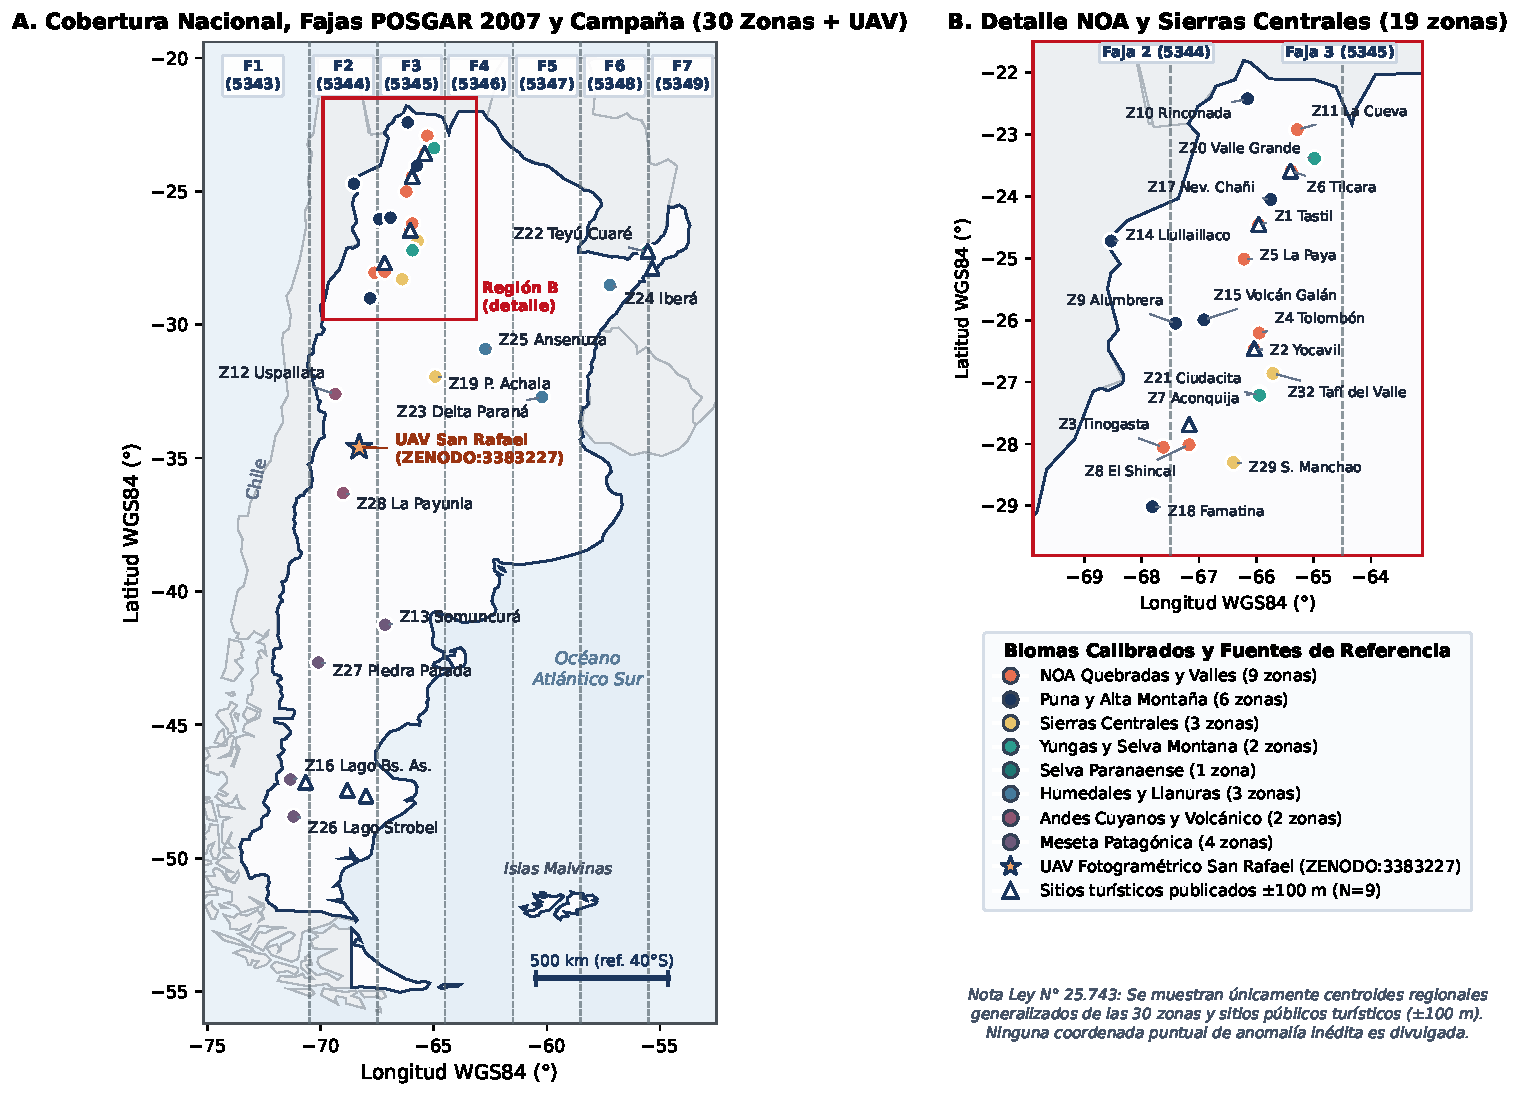
\includegraphics[width=0.95\textwidth]{figures/fig2_national_coverage_map.pdf}
\caption{Distribuci\'on geod\'esica de la campa\~na nacional \textbf{ArchaeoLiDAR-AR}. \textbf{A.} Territorio argentino segmentado en las siete fajas Gauss-Kr\"uger de POSGAR 2007 (\texttt{EPSG:5343--5349}, l\'ineas discontinuas verticales), mostrando los centroides regionales generalizados de las $30$ zonas objetivo (\texttt{TARGET\_ZONES}) coloreados por macro-bioma, el relevamiento fotogram\'etrico UAV de San Rafael (\texttt{ZENODO:3383227}) y los $9$ sitios tur\'isticos de dominio p\'ublico ($\pm 100\,\mathrm{m}$) del cat\'alogo \texttt{known\_sites\_published.csv}. \textbf{B.} Detalle de la regi\'on Noroeste y Sierras Centrales ($19$ zonas entre Faja 2 y Faja 3). Conforme a la Ley N\textsuperscript{o}~25.743, no se divulgan coordenadas puntuales de candidatos in\'editos.}
\label{fig:map}
\end{figure}

% ==================== SECTION 3 ====================
\FloatBarrier
\section{Metodolog\'ia Matem\'atica, Detecci\'on Morfom\'etrica y Calibraci\'on Epist\'emica}

\subsection{Modelos de Relieve \emph{NaN-Safe} y Trazabilidad de Par\'ametros}

Para suprimir la topograf\'ia macro-regional (laderas serranas, valles intermontanos y cordones cordilleranos) preservando anomal\'ias locales discretas, \texttt{src/core/relief\_models.py} implementa cuatro derivadas raster con manejo estricto de valores inv\'alidos (\texttt{NoData = -9999.0} convertido a \texttt{NaN} previo al c\'alculo):

\begin{enumerate}
  \item \textbf{Simple Local Relief Model (SLRM) normalizado por pesos:} Siguiendo la formulaci\'on de \citet{Hesse2010}, pero evitando anillos artificiales en los bordes de vac\'ios \emph{NoData} mediante convoluci\'on normalizada sobre la m\'ascara v\'alida $M(x,y) \in \{0,1\}$:
  \begin{equation}
  \mathrm{DTM}_{\mathrm{smooth}}(x,y) = \frac{\left(G_{\sigma} * (\mathrm{DTM}\cdot M)\right)(x,y)}{\left(G_{\sigma} * M\right)(x,y)}, \qquad \sigma = \max\!\left(1{,}0,\; \frac{R_{\mathrm{SLRM}}}{2\,\Delta s}\right),
  \label{eq:slrm_trend}
  \end{equation}
  \begin{equation}
  \mathrm{SLRM}(x,y) = \mathrm{DTM}(x,y) - \mathrm{DTM}_{\mathrm{smooth}}(x,y),
  \label{eq:slrm}
  \end{equation}
  donde $\Delta s = (\Delta x + \Delta y)/2$ es la resoluci\'on m\'etrica de grilla, $R_{\mathrm{SLRM}}$ es el radio caracter\'istico calibrado por bioma y los p\'ixeles con denominador $(G_\sigma * M) \le 10^{-6}$ o fuera de $M$ permanecen como \texttt{NaN}.
  \item \textbf{Pendiente topogr\'afica (\emph{Slope}):} Calculada en grados sexagesimales $[0^\circ, 90^\circ]$ mediante diferencias finitas centradas escaladas al paso m\'etrico real $(\Delta y, \Delta x)$:
  \begin{equation}
  S(x,y) = \arctan\!\left(\sqrt{\left(\frac{\partial\,\mathrm{DTM}}{\partial x}\right)^{\!2} + \left(\frac{\partial\,\mathrm{DTM}}{\partial y}\right)^{\!2}}\right) \cdot \frac{180^\circ}{\pi}.
  \label{eq:slope}
  \end{equation}
  \item \textbf{Sky-View Factor (SVF) y Openness Positivo/Negativo sin envolvimiento de bordes:} Implementados seg\'un \citet{Zaksek2011}, \citet{Yokoyama2002} y las buenas pr\'acticas de \citet{KokaljHesse2017}. A diferencia de implementaciones por desplazamiento circular (\texttt{np.roll}), el operador \texttt{\_shift\_no\_wrap\_nan} rellena fuera de l\'imite con \texttt{NaN}, impidiendo que el borde oeste contamine al este. Sobre $N_\theta = 16$ acimutes uniformes $\theta_k \in [0, 2\pi)$ y ventana radial truncada en pasos discretos $s \in [1, \min(12, \max(2, \mathrm{round}(R/\Delta s)))]$, se calcula el \'angulo m\'aximo de horizonte $\gamma_k = \max_s \arctan_2(\max(0, \mathrm{DTM}_{k,s} - \mathrm{DTM}), d_{k,s})$ para obtener $\mathrm{SVF} = \frac{1}{N_\theta}\sum_{k=1}^{N_\theta} (1 - \sin\gamma_k) \in [0, 1]$. De modo an\'alogo, con $N_\theta = 8$ direcciones y registrando los \'angulos extremos con signo $\beta_k = \max_s \alpha_{k,s}$ (cenital m\'aximo hacia arriba) y $\delta_k = \min_s \alpha_{k,s}$ (cenital m\'inimo hacia abajo), se obtienen \emph{Positive Openness} ($\mathrm{PO} = \frac{1}{8}\sum_k (90^\circ - \beta_k)$) y \emph{Negative Openness} ($\mathrm{NO} = \frac{1}{8}\sum_k (90^\circ + \delta_k)$), invariantes a la direcci\'on solar. Cada corrida persiste un archivo \emph{sidecar} (\texttt{*\_relief\_params.json}) con estad\'isticos y trazabilidad completa de par\'ametros.
\end{enumerate}

\subsection{Calibraci\'on Adaptativa por Bioma y Detecci\'on Morfom\'etrica en Doble Signo}

El territorio argentino demanda parametrizaciones geomorfol\'ogicas diferenciadas para prevenir tanto la p\'erdida de estructuras sutiles en llanuras como la explosi\'on de falsas alarmas en relieves abruptos. La Tabla~\ref{tab:biomes} detalla los ocho perfiles de calibraci\'on implementados en el sistema, distinguiendo el par\'ametro morfol\'ogico objetivo solicitado para fuentes sub-m\'etricas del piso f\'isico efectivo impuesto cuando la fuente de entrada es satelital de $30\,\mathrm{m/px}$.

\begin{table}[htbp]
\centering
\caption{Par\'ametros morfom\'etricos calibrados por macro-bioma argentino y piso f\'isico efectivo por resoluci\'on.}
\label{tab:biomes}
\footnotesize
\begin{tabularx}{\textwidth}{L{2.9cm} L{2.8cm} c c c c Y}
\toprule
\textbf{Macro-Bioma} & \textbf{Zonas Repres.} & $R_{\mathrm{SLRM}}$ & $A_{\min}$--$A_{\max}$ & $|\Delta z|_{\min}$ & $S_{\max}$ & \textbf{Objetivo Morfol\'ogico (Pases $+$ y $-$)} \\
 & & \textbf{(m)} & \textbf{(m$^2$)} & \textbf{(m)} & \textbf{($^\circ$)} & \\
\midrule
Alta Monta\~na y Puna & Cha\~ni, Llullaillaco, Famatina, Gal\'an & $12{,}0$ & $15$--$2000^\dagger$ & $0{,}30$ & $32$ & Plataformas cimeras, \emph{kanchas}, tambos y tramos del \emph{Qhapaq \~Nan}. \\
Yungas y Ceja de Selva & Valle Grande, Ciudacita & $15{,}0$ & $30$--$5000^\dagger$ & $0{,}35$ & $35$ & Andener\'ia prehisp\'anica, pucar\'as en filos y calzadas empedradas. \\
Sierras Centrales & Pampa de Achala, Manchao, Taf\'i & $10{,}0$--$15{,}0$ & $12$--$4000^\dagger$ & $0{,}20$--$0{,}25$ & $25$ & Casas-pozo semi-enterradas ($-$), pircas y corrales l\'iticos ($+$). \\
Selva Paranaense & Tey\'u Cuar\'e (Misiones) & $20{,}0$ & $50$--$6000^\dagger$ & $0{,}30$ & $25$ & Estructuras jesu\'itico-guaran\'ies bajo dosel, plataformas ($+$) y zanjas ($-$). \\
Humedales y Llanuras & Delta del Paran\'a, Iber\'a, Ansenuza & $35{,}0$--$40{,}0$ & $150$--$9000^\dagger$ & $0{,}25$--$0{,}35$ & $8$--$10$ & Cerritos y t\'umulos de tierra Goya-Malabrigo / Chan\'a-Timb\'u ($+$). \\
Meseta Patag\'onica & Lago Strobel, Piedra Parada, Somuncur\'a & $8{,}0$ & $6$--$500^\dagger$ & $0{,}25$ & $20$--$22$ & Parapetos circulares de caza de guanaco y \emph{chenques} de piedra ($+$). \\
Volc\'anico / Bas\'altico & La Payunia (Mendoza) & $10{,}0$ & $10$--$600^\dagger$ & $0{,}25$ & $25$ & Apostaderos y corrales l\'iticos emplazados sobre coladas bas\'alticas. \\
UAV Sub-m\'etrico & Vuelos de Dron ($\le 0{,}15\,\mathrm{m/px}$) & $2{,}5$--$6{,}0$ & $1{,}0$--$300$ & $0{,}10$ & $35$ & Muros individuales, cimientos, trincheras ($-$) y pedestales centim\'etricos. \\
\bottomrule
\multicolumn{7}{l}{\scriptsize $^\dagger$ Cuando el sensor activo es satelital global ($30\,\mathrm{m/px}$), el detector eleva autom\'aticamente $A_{\min,\mathrm{eff}} = \max(A_{\min}, 2\cdot 30^2) = 1800\,\mathrm{m}^2$.}
\end{tabularx}
\end{table}

El detector geom\'etrico (\texttt{src/core/anomaly\_detector.py}) subdivide cada raster maestro en celdas m\'etricas de $500\times 500\,\mathrm{m}$ con $15\%$ de solapamiento y ejecuta dos pases sim\'etricos de polaridad sobre la se\~nal acotada $s\cdot \mathrm{SLRM}(x,y)$ ($s \in \{+1, -1\}$) recortada al intervalo $[0, 3{,}0\,\mathrm{m}]$ y cuantizada a 8 bits:
\begin{enumerate}
  \item \textbf{Preservaci\'on de bordes y umbralizaci\'on adaptativa:} Aplica un filtro bilateral preservador de discontinuidades ($d=7$, $\sigma_{\mathrm{color}} = \sigma_{\mathrm{space}} = 35$), seguido de umbralizaci\'on adaptativa gaussiana (\texttt{blockSize}=31, $C=-2$), intersecci\'on con la m\'ascara f\'isica $[\Delta z_{\min}, 3{,}0\,\mathrm{m}] \cap \{S \le S_{\max}\} \cap M$ y clausura morfol\'ogica el\'iptica de $3\times 3\,\mathrm{px}$.
  \item \textbf{Control estricto de bordes y piso f\'isico:} Los contornos de relieve negativo ($s=-1$) que intersectan un margen de borde $\ge 2\,\mathrm{px}$ se descartan sistem\'aticamente, eliminando cauces y vaguadas pasantes para retener \'unicamente depresiones cerradas contenidas en la celda; el solapamiento del $15\%$ entre ventanas asegura la detecci\'on de depresiones pr\'oximas al l\'imite desde la celda adyacente. Toda poligonal cuya \'area corregida por discretizaci\'on de medio p\'ixel,
  \begin{equation}
  A_{\mathrm{eff}} = \left(A_{\mathrm{px}} + 0{,}5\,P_{\mathrm{px}}\right)\,\Delta x\,\Delta y,
  \label{eq:area_corr}
  \end{equation}
  resulte inferior al piso f\'isico $A_{\min,\mathrm{eff}} = \max(A_{\min,\mathrm{bioma}}, 2{,}0 \cdot \Delta x\,\Delta y)$ (constante \texttt{MIN\_AREA\_PIXEL\_FACTOR} $= 2{,}0$ evaluada sobre la resoluci\'on nativa del producto), se suprime y queda documentada en los metadatos de corrida (\texttt{min\_area\_floor\_applied}).
  \item \textbf{Descriptores morfol\'ogicos, deduplicaci\'on y desacoplamiento sem\'antico:} Se calculan rectangularidad ($\rho = A_{\mathrm{eff}} / A_{\mathrm{minRect}}$), circularidad isoperim\'etrica ($\gamma = 4\pi A_{\mathrm{eff}} / P^2$) y raz\'on de aspecto ($r_{\mathrm{asp}} = L/W$), clasificando preliminarmente cinco tipolog\'ias (\texttt{terraza\_lineal}, \texttt{estructura\_circular}, \texttt{recinto\_ortogonal}, \texttt{zanja\_lineal} y \texttt{estructura\_hundida}). Los duplicados en zonas de solapamiento se consolidan mediante b\'usqueda espacial exacta \texttt{scipy.spatial.cKDTree} con radio de supresi\'on de $30\,\mathrm{m}$ en POSGAR 2007. Crucialmente, cada pol\'igono incorpora el bloque estructurado \texttt{observable\_evidence} con la etiqueta expl\'icita \texttt{score\_interpretation} fijada en \texttt{\textquotedbl{}geometric\_topographic\_salience\_not\_archaeological\_probability\textquotedbl{}}, impidiendo confundir prominencia geom\'etrica con probabilidad arqueol\'ogica.
\end{enumerate}

\subsection{Validaci\'on Multifuente, Vigilancia de Saqueo (\texttt{ALERTA\_SAQUEO}) y Contexto \'Optico}

En Fase 3, \texttt{spatial\_validator.py} y \texttt{literature\_checker.py} contrastan cada candidato contra: (i) el servicio WFS del Instituto Geogr\'afico Nacional (\texttt{ign:linea\_de\_agua} e \texttt{ign:puntos\_de\_asentamientos\_y\_edificios}), midiendo distancias m\'etricas en POSGAR 2007; (ii) OpenStreetMap v\'ia Overpass API en un radio de $150\,\mathrm{m}$ (\texttt{historic=*}, \texttt{barrier=wall|fence}, \texttt{building=*}); (iii) el GeoPackage curado de sitios p\'ublicos (\texttt{known\_sites.gpkg}, $200\,\mathrm{m}$ de tolerancia sobre coordenadas aproximadas $\pm 100\,\mathrm{m}$); y (iv) antecedentes bibliogr\'aficos en OpenAlex y Semantic Scholar. De este cruce emergen tres clases preliminares: \texttt{SITIO\_REGISTRADO}, \texttt{FALSO\_POSITIVO\_MODERNO} y \texttt{CANDIDATO\_INEDITO}.

Simult\'aneamente, inspirado en la detecci\'on satelital de saqueo arqueol\'ogico de \citet{Parcak2016}, el m\'odulo \texttt{looting\_monitor.py} activa autom\'aticamente la bandera \texttt{patrimonial\_priority = \textquotedbl{}ALERTA\_SAQUEO\textquotedbl{}} cuando concurren cinco condiciones: relieve negativo neto ($\Delta z < 0$, \texttt{estructura\_hundida}), morfolog\'ia circular ($\gamma \ge 0{,}5$, $r_{\mathrm{asp}} \le 1{,}6$), di\'ametro equivalente $D_{\mathrm{eq}} = 2\sqrt{A/\pi} \in [5, 25]\,\mathrm{m}$, y proximidad $< 1000\,\mathrm{m}$ respecto de un sitio del cat\'alogo o contexto patrimonial/edificado en OSM o IGN. Esta alerta inyecta una secci\'on de denuncia urgente (arts.\ 20 y 23, Ley N\textsuperscript{o}~25.743) en el dossier INAPL correspondiente.

\'Unicamente sobre candidatos \texttt{CANDIDATO\_INEDITO}, la Fase 4 (\texttt{optical\_providers.py}) descarga un chip multiespectral centrado ($\pm 150\,\mathrm{m}$, tope $512\times 512\,\mathrm{px}$) de Sentinel-2 L2A u ortomosaicos XYZ/IGN Argenmap, calculando $\mathrm{NDVI} = (\mathrm{B08}-\mathrm{B04})/(\mathrm{B08}+\mathrm{B04})$, $\mathrm{NDWI} = (\mathrm{B03}-\mathrm{B08})/(\mathrm{B03}+\mathrm{B08})$ y el contraste diferencial $\Delta\mathrm{NDVI} = \overline{\mathrm{NDVI}}_{\mathrm{interior}} - \overline{\mathrm{NDVI}}_{\mathrm{anillo}}$ para detectar \emph{cropmarks} asociados a muros enterrados o alteraci\'on ed\'afica.

\subsection{Inspecci\'on Multimodal, Juez Pericial VLM, Calibrador ML y Regla de Abstenci\'on}

El m\'odulo \texttt{visual\_inspector.py} junto con \texttt{src/utils/blender\_render.py} genera l\'aminas compuestas de 4 paneles ($2\times 2$) o 6 paneles ($2\times 3$): (1) \emph{Hillshade} multidireccional ($4$ acimutes $315^\circ, 45^\circ, 135^\circ, 225^\circ$, exageraci\'on $1{,}5\times$), (2) mapa SLRM en paleta divergente/viridis, (3) perfil topogr\'afico 2D sobre el centroide en POSGAR 2007, (4) renderizado volum\'etrico isom\'etrico en Blender 4.2 LTS EEVEE ($1{,}8\times$ de exageraci\'on vertical, con conmutaci\'on segura a mapa DTM 2D si Blender no est\'a disponible), (5) RGB satelital y (6) mapa espectral NDVI con el contorno candidato superpuesto.

Sobre estas l\'aminas opera el Juez Pericial Multimodal (\texttt{vlm\_judge.py}), siguiendo el paradigma estructurado \emph{LLM-as-a-Judge} \citep{Zheng2023} bajo criterios geomorfol\'ogicos del NOA/CONICET. Todo dictamen de descarte (\texttt{NATURAL} o \texttt{ARTEFACTO}) ejecuta una purga at\'omica v\'ia \texttt{record\_vlm\_verdict()}: remueve la geometr\'ia de \texttt{MAPA\_FINAL\_PROSPECCION.geojson} y \texttt{MAPA\_PROSPECCION\_*.geojson}, registra la justificaci\'on forense en \texttt{DESCARTES\_VLM.json} y alimenta \texttt{INVENTARIO\_GEOMORFOLOGICO.geojson} con su subtipo geol\'ogico.

Para priorizar candidatos antes del juicio visual y siguiendo las estrategias supervisadas multi-escala de \citet{Guyot2018} y \citet{BerganzoBesga2021}, \texttt{src/core/ml\_calibrator.py} entrena un clasificador \texttt{GradientBoostingClassifier} ($150$ \'arboles, profundidad m\'axima $3$, tasa de aprendizaje $0{,}08$) envuelto en imputaci\'on por mediana (\texttt{SimpleImputer}) y calibraci\'on probabil\'istica isot\'onica (\texttt{CalibratedClassifierCV}, $3$ particiones internas) sobre un vector de $11$ variables geom\'etricas, contextuales de ventana ($r=75\,\mathrm{m}$) y espectrales: \texttt{area\_m2}, \texttt{dz\_mean}, \texttt{dz\_abs}, \texttt{rectangularity}, \texttt{circularity}, \texttt{aspect\_ratio}, \texttt{dz\_extreme\_window}, \texttt{slope\_mean\_deg}, \texttt{slrm\_std\_window}, \texttt{dz\_contrast\_ratio} y \texttt{ndvi\_anomaly\_delta}. La evaluaci\'on se efect\'ua mediante validaci\'on cruzada estratificada agrupada por zona/fuente (\texttt{StratifiedGroupKFold}, $5$ particiones) para evitar fuga por autocorrelaci\'on espacial \citep{Roberts2017}.

Finalmente, la Etapa~3 integra la compuerta determinista de abstenci\'on \texttt{should\_abstain\_prediction()} en \texttt{benchmark\_v1.py}, que transiciona el candidato al estado formal \texttt{INCONCLUSIVE} cuando se satisface cualquiera de cuatro criterios objetivos:
\begin{enumerate}
  \item El raster de entrada posee marca \texttt{SYNTHETIC\_FALLBACK} o nivel \texttt{SYNTHETIC\_UNSUITABLE};
  \item La fracci\'on de vac\'ios inv\'alidos supera el umbral cr\'itico (\texttt{void\_fraction} $> 0{,}25$);
  \item El \'area del rasgo candidato es inferior al piso f\'isico del sensor ($A_{\mathrm{obj}} < 2 \cdot \mathrm{GSD}_{\mathrm{nativo}}^2$); o
  \item La probabilidad calibrada ML cae dentro de la banda operativa de incertidumbre $[0{,}35,\; 0{,}65]$.
\end{enumerate}
Ninguna evaluaci\'on autom\'atica (\texttt{AI\_PREASSESSMENT}) puede promoverse sin auditor\'ia externa al estado \texttt{EXPERT\_REVIEWED} ni a \texttt{FIELD\_CONFIRMED}, garantizando una separaci\'on ontol\'ogica de siete estados definida en \texttt{CandidateLifecycleState} (\texttt{src/schemas.py}).

% ==================== SECTION 4 ====================
\FloatBarrier
\section{Verificaci\'on del Motor, Resultados Emp\'iricos de Campa\~na y Benchmark ML}

\subsection{Auditor\'ia F\'isico-Geoespacial Determinista y Suite de Pruebas}

Previo al an\'alisis de campa\~na, la integridad num\'erica del motor fue verificada mediante una suite de $64$ pruebas autom\'aticas distribuidas en $13$ m\'odulos de prueba (\texttt{pytest}: $64/64$ aprobadas en $68{,}69\,\mathrm{s}$), incluyendo las $8$ pruebas f\'isico-geoespaciales obligatorias de \texttt{tests/test\_engine\_scientific\_audit.py} detalladas en la Tabla~\ref{tab:audit8}.

\begin{table}[htbp]
\centering
\caption{Resultados de la suite determinista de auditor\'ia cient\'ifica del motor (\texttt{test\_engine\_scientific\_audit.py}, $8/8$ aprobadas).}
\label{tab:audit8}
\footnotesize
\begin{tabularx}{\textwidth}{c L{3.6cm} L{5.1cm} Y}
\toprule
\textbf{\#} & \textbf{Prueba de Auditor\'ia} & \textbf{Condici\'on Experimental Sint\'etica} & \textbf{Invariante Verificado (Pasa)} \\
\midrule
1 & Recuperaci\'on en doble signo & Recinto $22\times 22\,\mathrm{m}$ ($+1{,}1\,\mathrm{m}$) y pozo $r=9\,\mathrm{m}$ ($-1{,}2\,\mathrm{m}$) a $1\,\mathrm{m/px}$ & Recupera ambos signos (\texttt{positive}/\texttt{negative}), SVF/Openness y metadatos \texttt{observable\_evidence}. \\
2 & Superficie plana y rampa uniforme & Plano constante ($2500\,\mathrm{m}$) y rampa $0{,}08x + 0{,}04y$ & $0$ anomal\'ias espurias generadas en SLRM ni OpenCV. \\
3 & Vac\'ios internos y bordes \emph{NoData} & Bloque central y bandas perimetrales en \texttt{NODATA\_FLOAT32} & Sin anillos artificiales en SLRM, SVF ($>0{,}99$ plano), Openness ni contornos ($0$ falsas detecciones). \\
4 & Degradaci\'on multi-resoluci\'on & Estructura de $16\times 16\,\mathrm{m}$ evaluada a $1\,\mathrm{m/px}$ vs.\ $30\,\mathrm{m/px}$ & Detectada a $1\,\mathrm{m/px}$ (\texttt{suitable=True}); bloqueada a $30\,\mathrm{m/px}$ con piso $A_{\min,\mathrm{eff}}=1800\,\mathrm{m}^2$. \\
5 & Consistencia entre fajas POSGAR & Estructura $30\times 30\,\mathrm{m}$ proyectada en Faja 2 (\texttt{5344}) vs.\ Faja 3 (\texttt{5345}) & Discrepancia relativa en \'area geom\'etrica $< 2\%$. \\
6 & Invariancia rotacional $90^\circ$ & Cuadrado $28\times 28\,\mathrm{m}$ vs.\ matriz rotada \texttt{np.rot90} & Anisotrop\'ia controlada en hillshade vs.\ invariancia en SLRM/SVF/Openness y \'area ($\le 2\%$). \\
7 & Robustez ante erosi\'on y ruido & Suavizado gaussiano ($\sigma=1{,}2$) + ruido normal ($\sigma=0{,}04\,\mathrm{m}$) & Conserva recuperaci\'on estable de la huella morfol\'ogica ($\ge 300\,\mathrm{m}^2$ sobre $784\,\mathrm{m}^2$). \\
8 & Determinismo bit-a-bit & Dos ejecuciones independientes id\'enticas sobre el mismo DTM & Salida geom\'etrica y atributos de \texttt{features} estrictamente id\'enticos. \\
\bottomrule
\end{tabularx}
\end{table}

\subsection{Reconciliaci\'on de Campa\~na, Auditor\'ia de Procedencia y Resultados sobre 121 Anomal\'ias}

La campa\~na exploratoria nacional recorri\'o $2.490$ cuadr\'iculas m\'etricas distribuidas en las $30$ zonas del cat\'alogo argentino m\'as relevamientos de alta resoluci\'on. En aras de la m\'axima transparencia cient\'ifica, la Tabla~\ref{tab:reconciliation} reconcilia de manera expl\'icita las dos instant\'aneas auditadas del repositorio: la l\'inea base congelada \texttt{baseline-v1.0} (\texttt{CAMPAIGN\_MANIFEST.json}, commit \texttt{0b0ffbd}, $N=126$ descartes) y el corpus vivo depurado por procedencia (\texttt{DESCARTES\_VLM.json}, $N=121$ anomal\'ias tras el commit \texttt{83dc82e} y la incorporaci\'on de \texttt{ARQ-TEY-0005}).

\begin{table}[htbp]
\centering
\caption{Reconciliaci\'on cuantitativa entre la l\'inea base congelada (\texttt{baseline-v1.0}) y el corpus vivo auditado por procedencia.}
\label{tab:reconciliation}
\footnotesize
\begin{tabularx}{\textwidth}{L{4.8cm} c c Y}
\toprule
\textbf{M\'etrica Consolidada} & \textbf{L\'inea Base \texttt{baseline-v1.0}} & \textbf{Corpus Vivo Depurado} & \textbf{Trazabilidad y Causa de Diferencia} \\
 & \textbf{(13-Nov-2026)} & \textbf{(14-Nov-2026)} & \\
\midrule
Zonas geogr\'aficas en cat\'alogo & $30$ & $30$ & Cat\'alogo \texttt{TARGET\_ZONES} (Fajas POSGAR 1--7). \\
Total de anomal\'ias auditadas (VLM) & $126$ & $121$ & Purga de $6$ registros \texttt{ARQ-HR-0001..0006} (Cascadia) + adici\'on de \texttt{ARQ-TEY-0005}. \\
Dictamen \texttt{NATURAL} (\texttt{REJECTED\_NATURAL}) & $103$ ($81{,}7\%$) & $98$ ($81{,}0\%$) & Purga de $6$ geoformas mal atribuidas + adici\'on de \texttt{ARQ-TEY-0005} (\texttt{NATURAL}, $89\%$). \\
Dictamen \texttt{ARTEFACTO} (\texttt{REJECTED\_MODERN}) & $23$ ($18{,}3\%$) & $23$ ($19{,}0\%$) & Costuras de tile, huellas modernas y pedestal \texttt{ARQ-HRM-0001} (San Rafael UAV). \\
Confirmadas en \texttt{MAPA\_FINAL\_PROSPECCION} & $0$ & $0$ & Regla estricta de cero falsos positivos enviados a terreno. \\
Geoformas en \texttt{INVENTARIO\_GEOMORFOLOGICO} & $86$ & $81$ & $6$ entradas mal atribuidas removidas + $1$ paleocauce/vaguada agregada (\texttt{ARQ-TEY-0005}). \\
Dossiers t\'ecnicos INAPL emitidos & $126$ & $121$ & Documentaci\'on forense individual (\texttt{DOSSIER\_INAPL\_*.md}). \\
Polaridad: relieve positivo / negativo & --- & $113$ / $8$ & Incluye $4$ \texttt{estructura\_hundida} y $4$ \texttt{zanja\_lineal} en corpus vivo. \\
\bottomrule
\end{tabularx}
\end{table}

Un hallazgo metodol\'ogico significativo surgido de la propia auditor\'ia del proyecto ocurri\'o al verificar la procedencia de los conjuntos externos descargados por el buscador autom\'atico (\texttt{HighResLidarHunter}): las $6$ anomal\'ias \texttt{ARQ-HR-0001..0006}, derivadas del registro \texttt{ZENODO:18023344}, resultaron corresponder a la falla geol\'ogica San Juan en Cascadia (Canad\'a) y no a la Precordillera de San Juan (Argentina). Tras la detecci\'on de esa homonimia topon\'imica, dichos registros y sus mapas fueron purgados en su totalidad (commit \texttt{83dc82e}), conservando \'unicamente el vuelo fotogram\'etrico argentino verificado de San Rafael, Mendoza (\texttt{ZENODO:3383227}, \citealp{Soderholm2019}). Este episodio demuestra el valor de mantener auditor\'ia de procedencia geod\'esica antes de incorporar conjuntos p\'ublicos al inventario patrimonial.

En el corpus vivo depurado ($N=121$), el $100\%$ de las anomal\'ias in\'editas preseleccionadas fue filtrado sin falsas derivaciones a terreno: $98$ ($81{,}0\%$) correspondieron a geoformas naturales y $23$ ($19{,}0\%$) a artefactos t\'ecnicos o estructuras contempor\'aneas (Figura~\ref{fig:campaign}). Morfom\'etricamente predominaron las terrazas lineales ($41$; $33{,}9\%$), estructuras circulares ($37$; $30{,}6\%$) y recintos ortogonales ($35$; $28{,}9\%$), complementadas por $8$ detecciones de relieve negativo ($4$ \texttt{estructura\_hundida} y $4$ \texttt{zanja\_lineal}; $6{,}6\%$). La amplitud vertical absoluta observada oscil\'o entre $0{,}200\,\mathrm{m}$ y $2{,}774\,\mathrm{m}$ (mediana $1{,}426\,\mathrm{m}$), la superficie en planta entre $1{,}2\,\mathrm{m}^2$ y $7877{,}9\,\mathrm{m}^2$ (mediana $567{,}5\,\mathrm{m}^2$; media $1008{,}2\,\mathrm{m}^2$), y la certeza pericial del Juez VLM promedi\'o $92{,}70\%$ (mediana $93{,}0\%$; rango $85\%$--$98\%$). Como subproducto cient\'ifico directo, $81$ descartes naturales quedaron catalogados en $11$ subtipos dentro de \texttt{INVENTARIO\_GEOMORFOLOGICO.geojson}, encabezados por domos volc\'anicos ($n=15$), albardones aluviales ($n=11$), lomadas ($n=9$), paleocauces ($n=9$), canchales ($n=8$) y morrenas ($n=8$).

\begin{figure}[htbp]
\centering
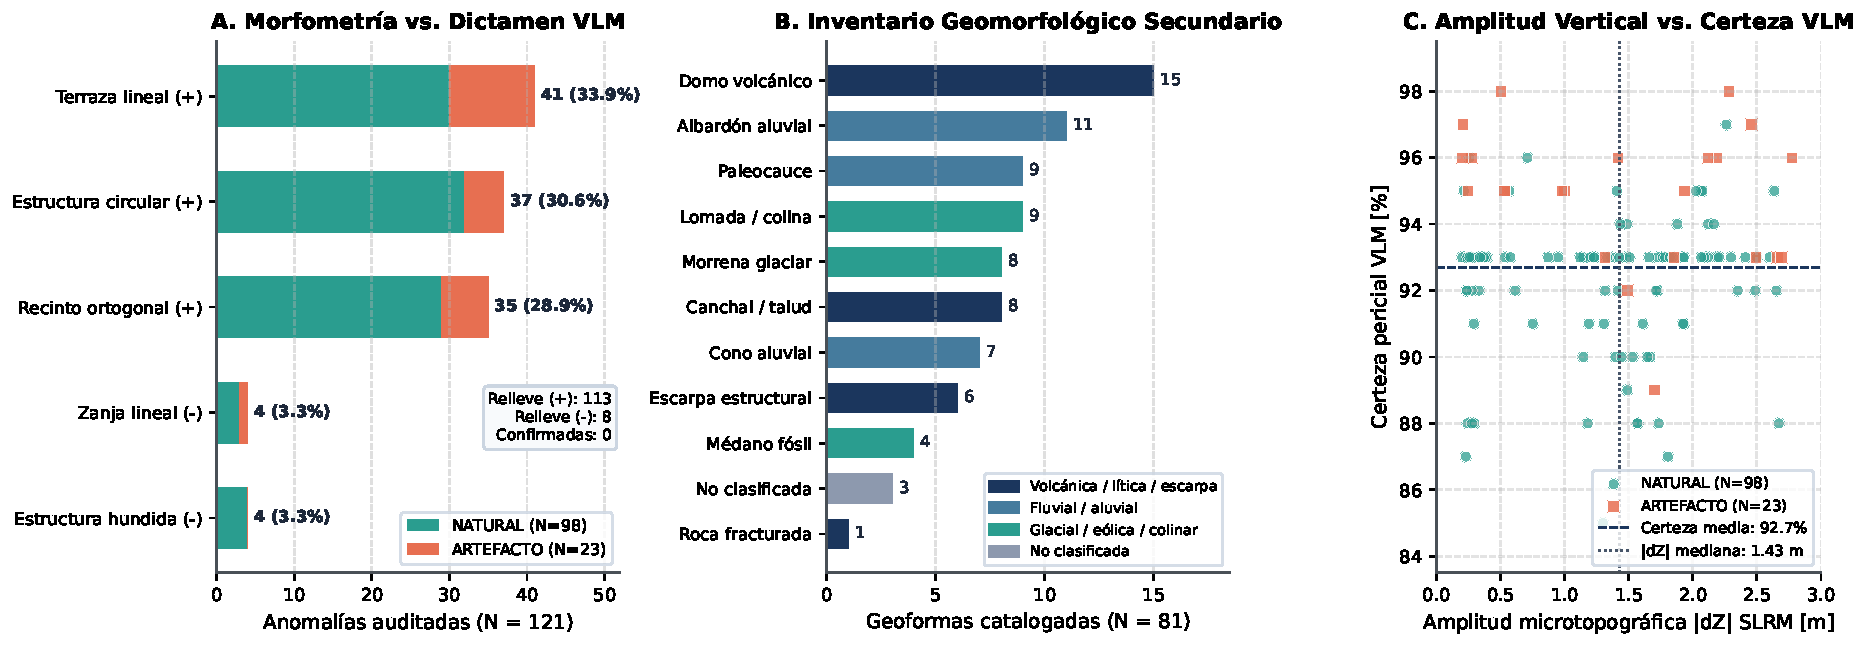
\includegraphics[width=\textwidth]{figures/fig4_campaign_results_and_geoforms.pdf}
\caption{Resultados emp\'iricos consolidados del corpus vivo auditado ($N=121$ anomal\'ias y $N=81$ geoformas secundarias). \textbf{A.} Distribuci\'on por tipolog\'ia morfom\'etrica en doble pase ($+$ y $-$) desglosada por dictamen pericial VLM (\texttt{NATURAL} vs.\ \texttt{ARTEFACTO}). \textbf{B.} Taxonom\'ia del inventario geomorfol\'ogico secundario derivado de los descartes naturales ($11$ subtipos). \textbf{C.} Relaci\'on entre amplitud vertical relativa $|\Delta z|$ del SLRM y certeza pericial asignada por el Juez Multimodal.}
\label{fig:campaign}
\end{figure}

\subsection{Casos de Estudio Multimodales: Descarte Positivo, Relieve Negativo Multisat\'elite y Artefacto UAV}

Para ilustrar c\'omo la integraci\'on de corte transversal, modelo 3D y contexto espectral previene falsos positivos en tres reg\'imenes f\'isicos opuestos, se documentan tres casos reales del repositorio:

\begin{enumerate}
  \item \textbf{Relieve negativo bajo selva subtropical (\texttt{ARQ-TEY-0005}, Pe\~n\'on del Tey\'u Cuar\'e, Misiones):} Detectado en pase negativo sobre FABDEM V1-2 (proyecci\'on m\'etrica POSGAR 2007, $\Delta z_{\mathrm{media}} = -1{,}49\,\mathrm{m}$, \'area $2763{,}48\,\mathrm{m}^2$, \texttt{zanja\_lineal}, raz\'on de aspecto $6{,}9$). Aunque el contexto regional contempla fosos y zanjas jesu\'itico-guaran\'ies bajo canopia, la l\'amina de 6 paneles (Figura~\ref{fig:teyu}) demuestra en el Panel 3 un perfil transversal monot\'onico en ``V'' abierta de $\sim 200\,\mathrm{m}$ de ancho y $\sim 2{,}4\,\mathrm{m}$ de profundidad sin paredes excavadas ni piso plano, un corredor c\'oncavo abierto en Blender 3D (Panel 4) y ausencia de \emph{cropmark} arquitect\'onico en Sentinel-2 ($\mathrm{NDVI}=0{,}8411$, $\Delta\mathrm{NDVI}=-0{,}0594$, $\mathrm{NDWI}=-0{,}754$, probabilidad ML $0{,}031$). El Juez Pericial dictamin\'o \texttt{NATURAL} con $89\%$ de certeza (vaguada de escorrent\'ia natural), incorpor\'andolo al inventario geomorfol\'ogico.
  \item \textbf{Falso recinto por sobremuestreo regional (\texttt{ARQ-MAN-0004}, Sierra de Manchao, Sierras Centrales):} Sobre Copernicus GLO-30 (\texttt{EPSG:5345}), el detector aisl\'o una elevaci\'on positiva centrada en una ladera serrana. La l\'amina de 4 paneles con renderizado t\'ermico EEVEE (Figura~\ref{fig:manchao}) evidencia flancos coluviales suaves de transici\'on continua sin rupturas angulares de paramento ni esquinas ortogonales, permitiendo su archivo como geoforma natural \texttt{NATURAL} y exponiendo las limitaciones morfol\'ogicas de grillas de $30\,\mathrm{m/px}$ frente a muros de pirca angostos.
  \item \textbf{Artefacto instrumental sub-m\'etrico a $5\,\mathrm{cm/px}$ (\texttt{ARQ-HRM-0001}, San Rafael, Mendoza, \texttt{ZENODO:3383227}):} A resoluci\'on fotogram\'etrica UAV centim\'etrica, el algoritmo segment\'o un pol\'igono hiper-rectangular de $1{,}24\,\mathrm{m}^2$ ($\text{rectangularidad}=0{,}7351$, $\Delta z = +0{,}503\,\mathrm{m}$, confianza morfol\'ogica $0{,}866$). El perfil 2D y el modelo volum\'etrico en Blender 4.2 (Figura~\ref{fig:hailpixel}) revelan un prisma recto de $1{,}2\times 0{,}8\,\mathrm{m}$ con paredes verticales a $90^\circ$ emplazado junto a estr\'ias paralelas de rodado vehicular: corresponde a la mesa de calibraci\'on meteorol\'ogica (\emph{hail pad}) del experimento HailPixel \citep{Soderholm2019}. Fue dictaminado \texttt{ARTEFACTO} con $98\%$ de certeza y purgado del mapa patrimonial.
\end{enumerate}

\begin{figure}[htbp]
\centering
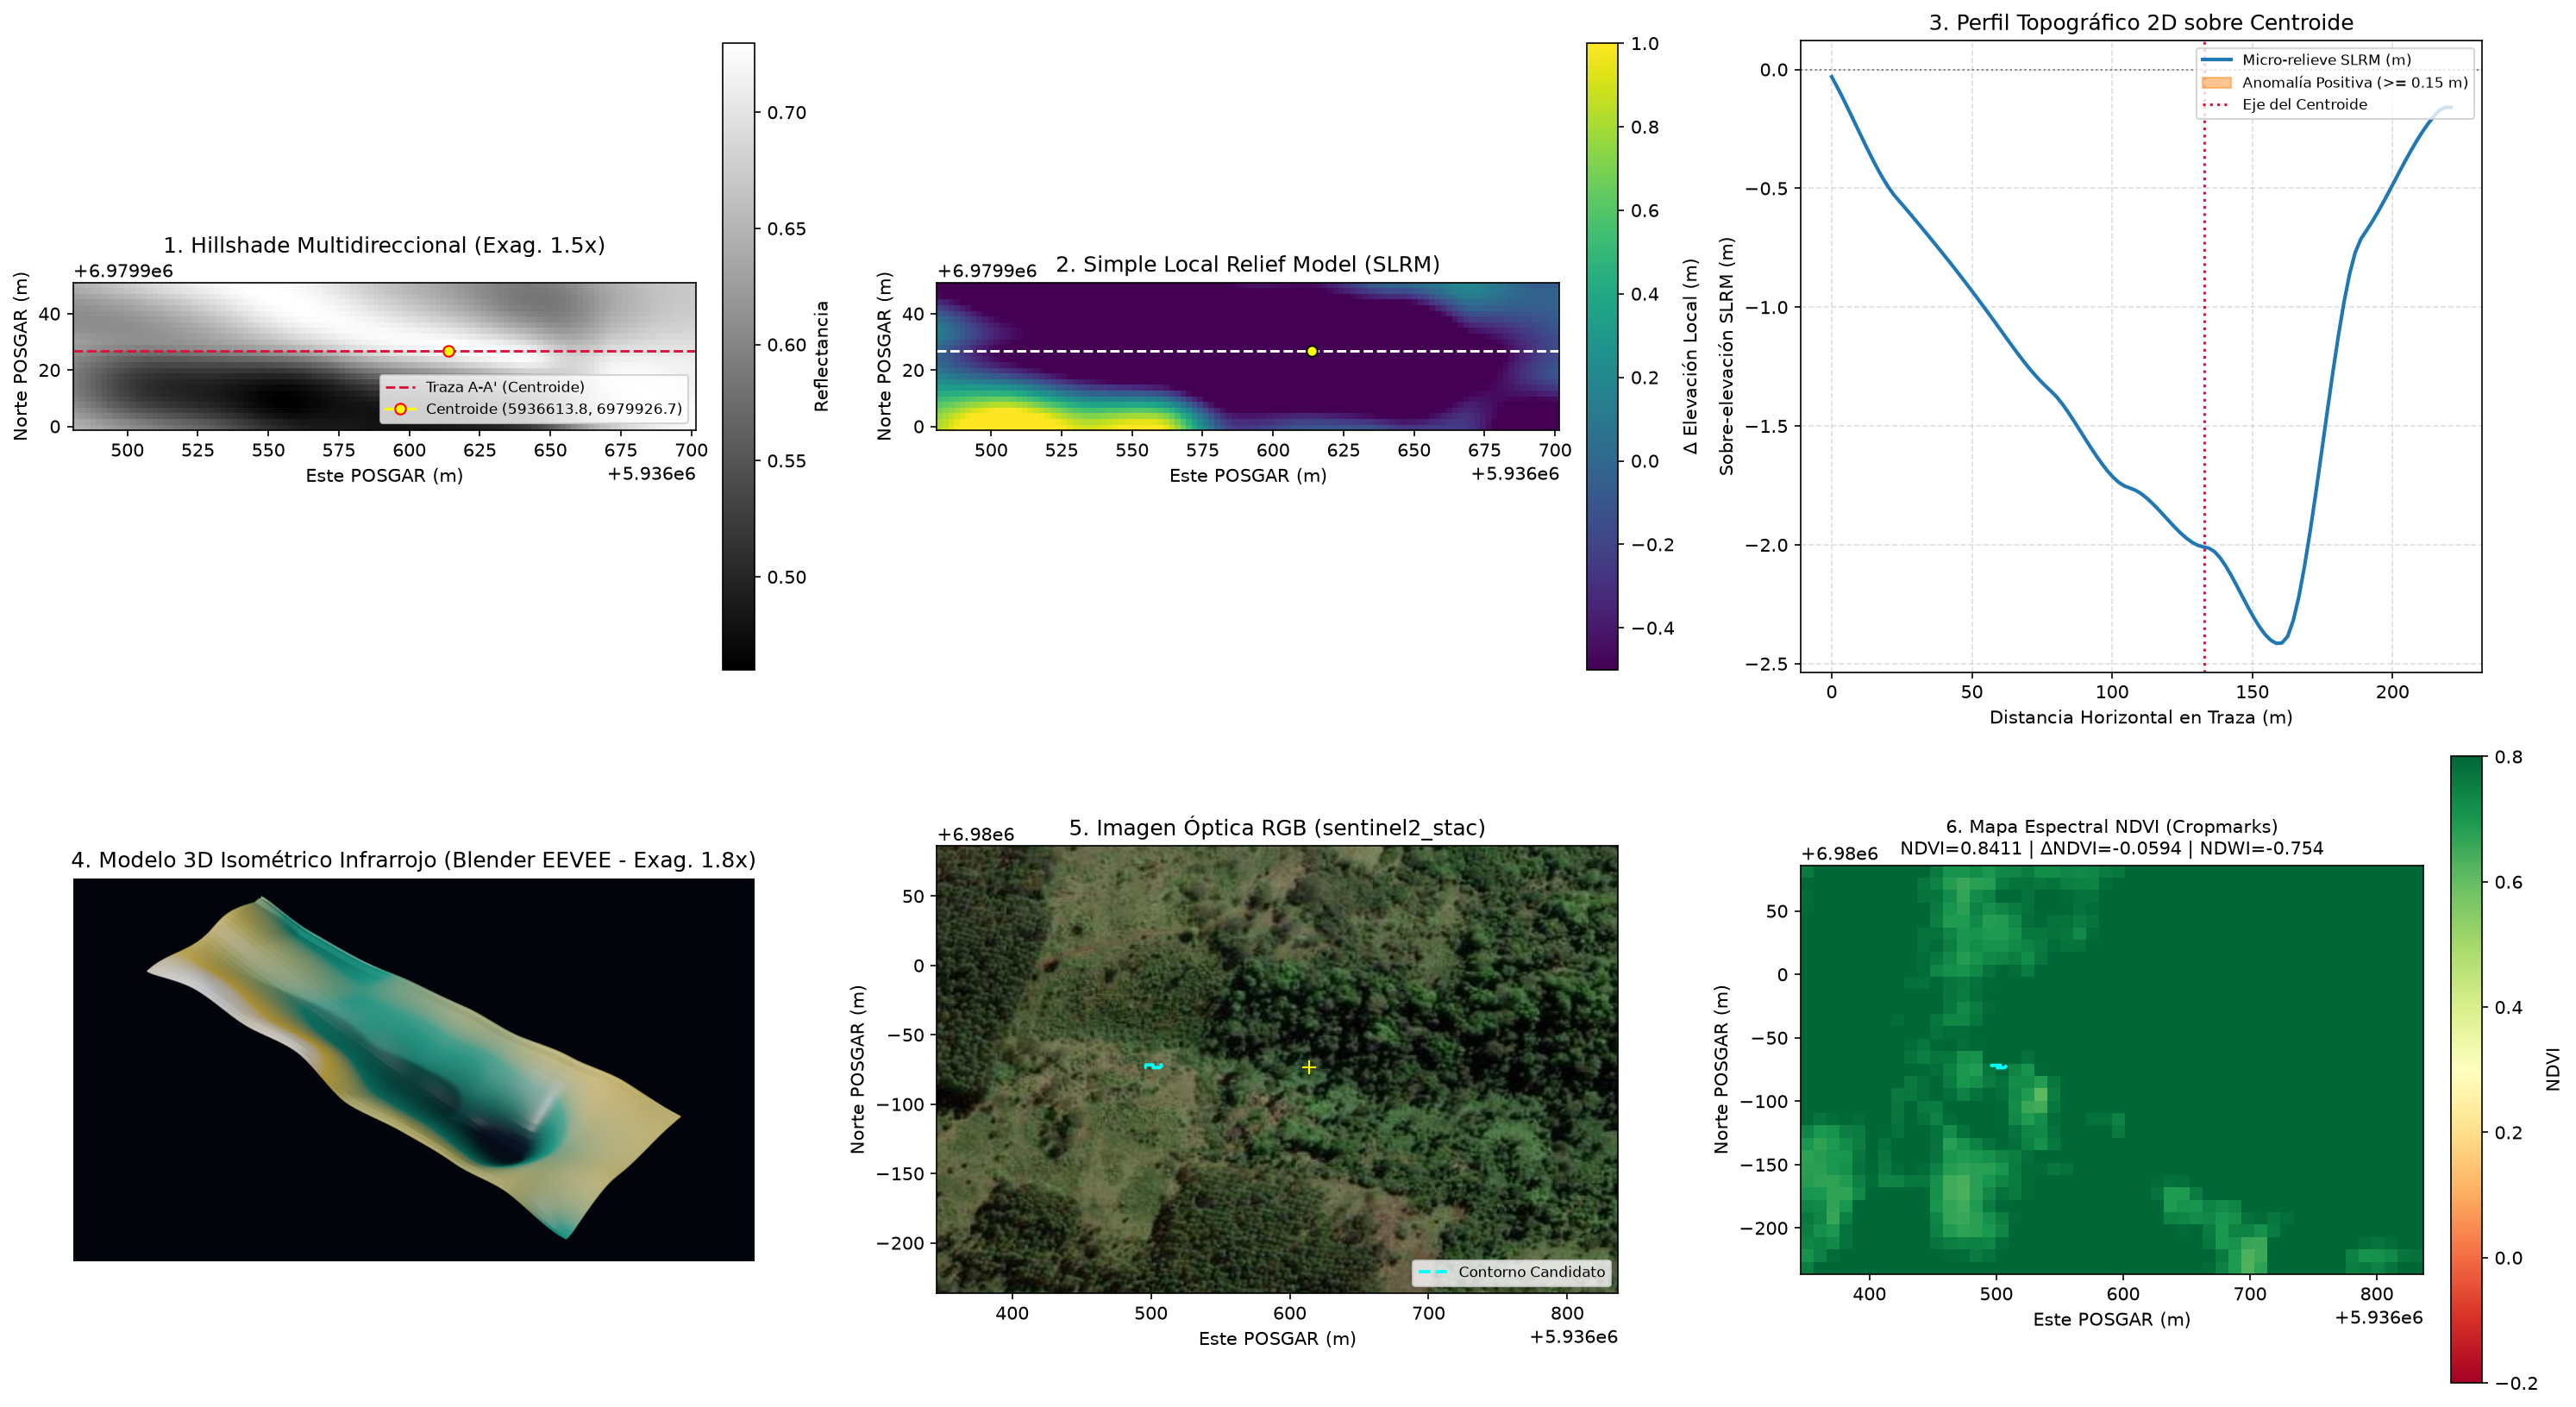
\includegraphics[width=0.90\textwidth]{figures/fig5_teyu_cuare_6panel.png}
\caption{Caso de estudio en relieve negativo y selva subtropical: l\'amina multimodal de 6 paneles para el candidato descartado \texttt{ARQ-TEY-0005} (\texttt{ZONA\_22\_TEYU\_CUARE}, Misiones, FABDEM + Sentinel-2 L2A). Los paneles integran \emph{Hillshade} multidireccional ($1{,}5\times$), SLRM, perfil transversal 2D en ``V'' abierta ($\sim 200\,\mathrm{m}$ de ancho), render 3D Blender 4.2 EEVEE ($1{,}8\times$), RGB Sentinel-2 y NDVI ($\mathrm{NDVI}=0{,}8411$, $\Delta\mathrm{NDVI}=-0{,}0594$). Dictamen pericial: \textbf{NATURAL} (vaguada natural de escorrent\'ia, certeza $89\%$).}
\label{fig:teyu}
\end{figure}

\begin{figure}[htbp]
\centering
\begin{subfigure}[t]{0.72\textwidth}
  \centering
  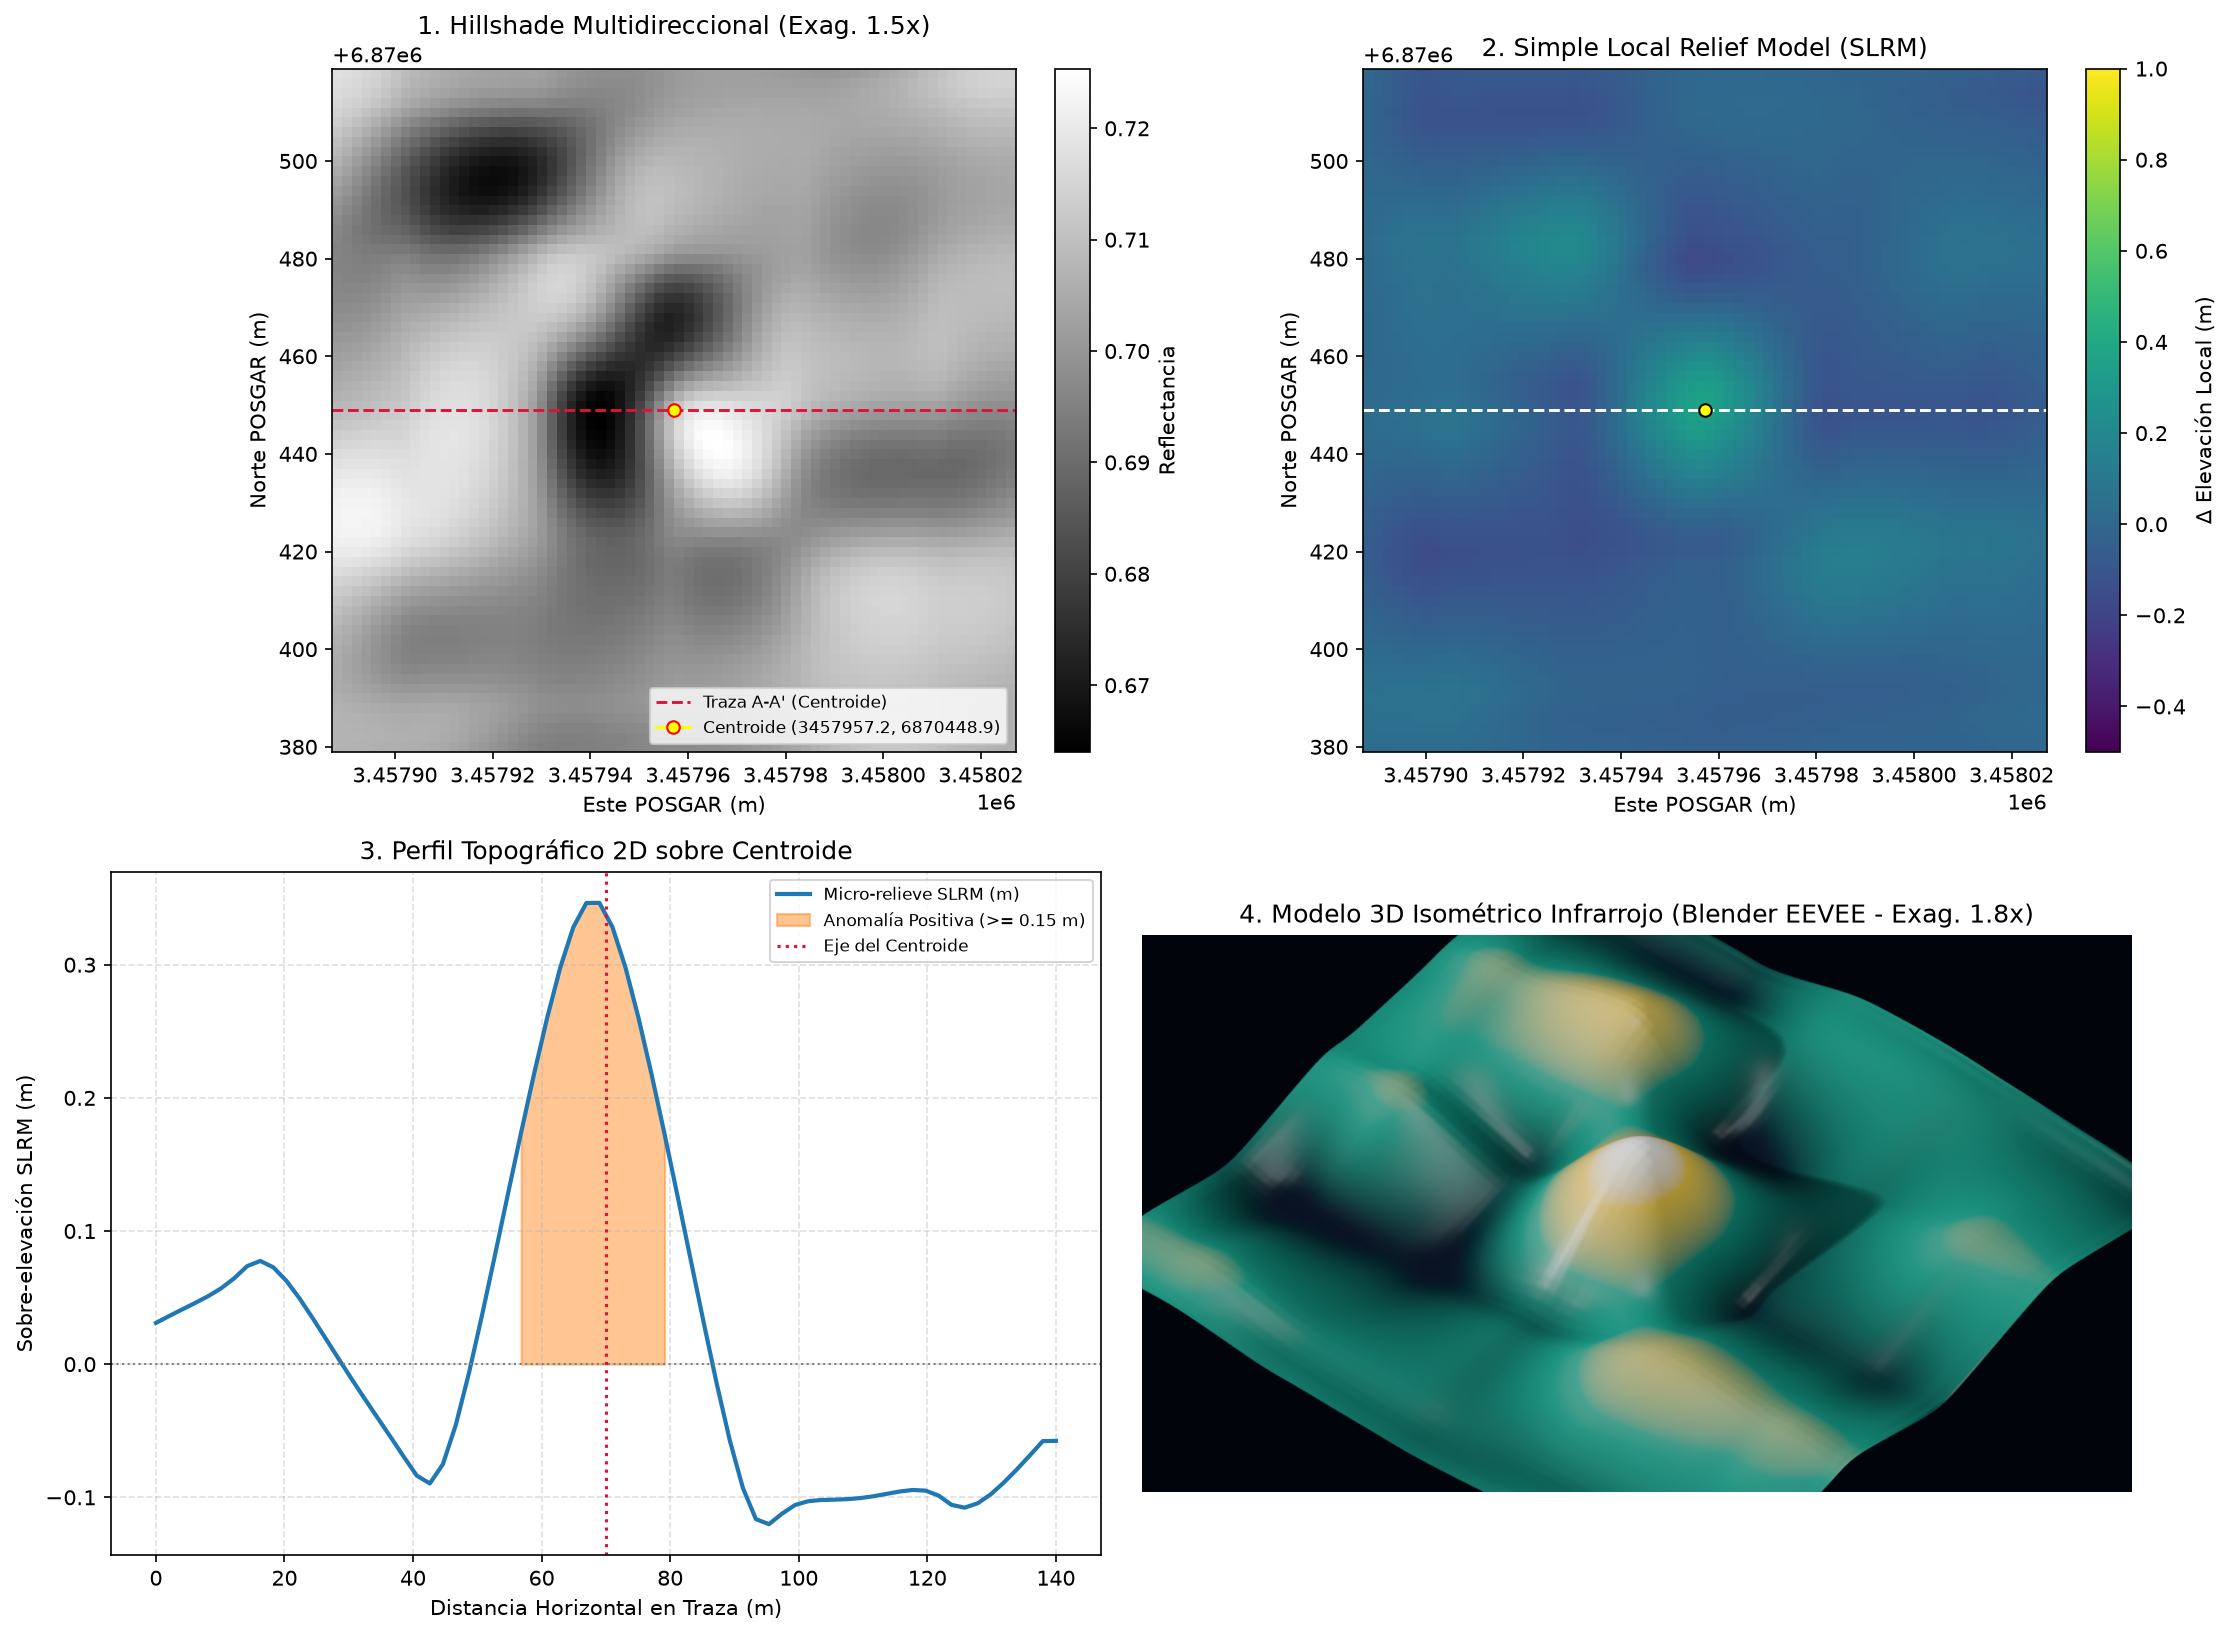
\includegraphics[width=\textwidth]{figures/fig6a_manchao_4panel.png}
  \caption{Caso regional $30\,\mathrm{m/px}$ (\texttt{ARQ-MAN-0004}, Sierra de Manchao): domo coluvial continuo sin paramentos ortogonales en corte 2D ni render Blender (\textbf{NATURAL}).}
  \label{fig:manchao}
\end{subfigure}

\vspace{6pt}
\begin{subfigure}[t]{0.72\textwidth}
  \centering
  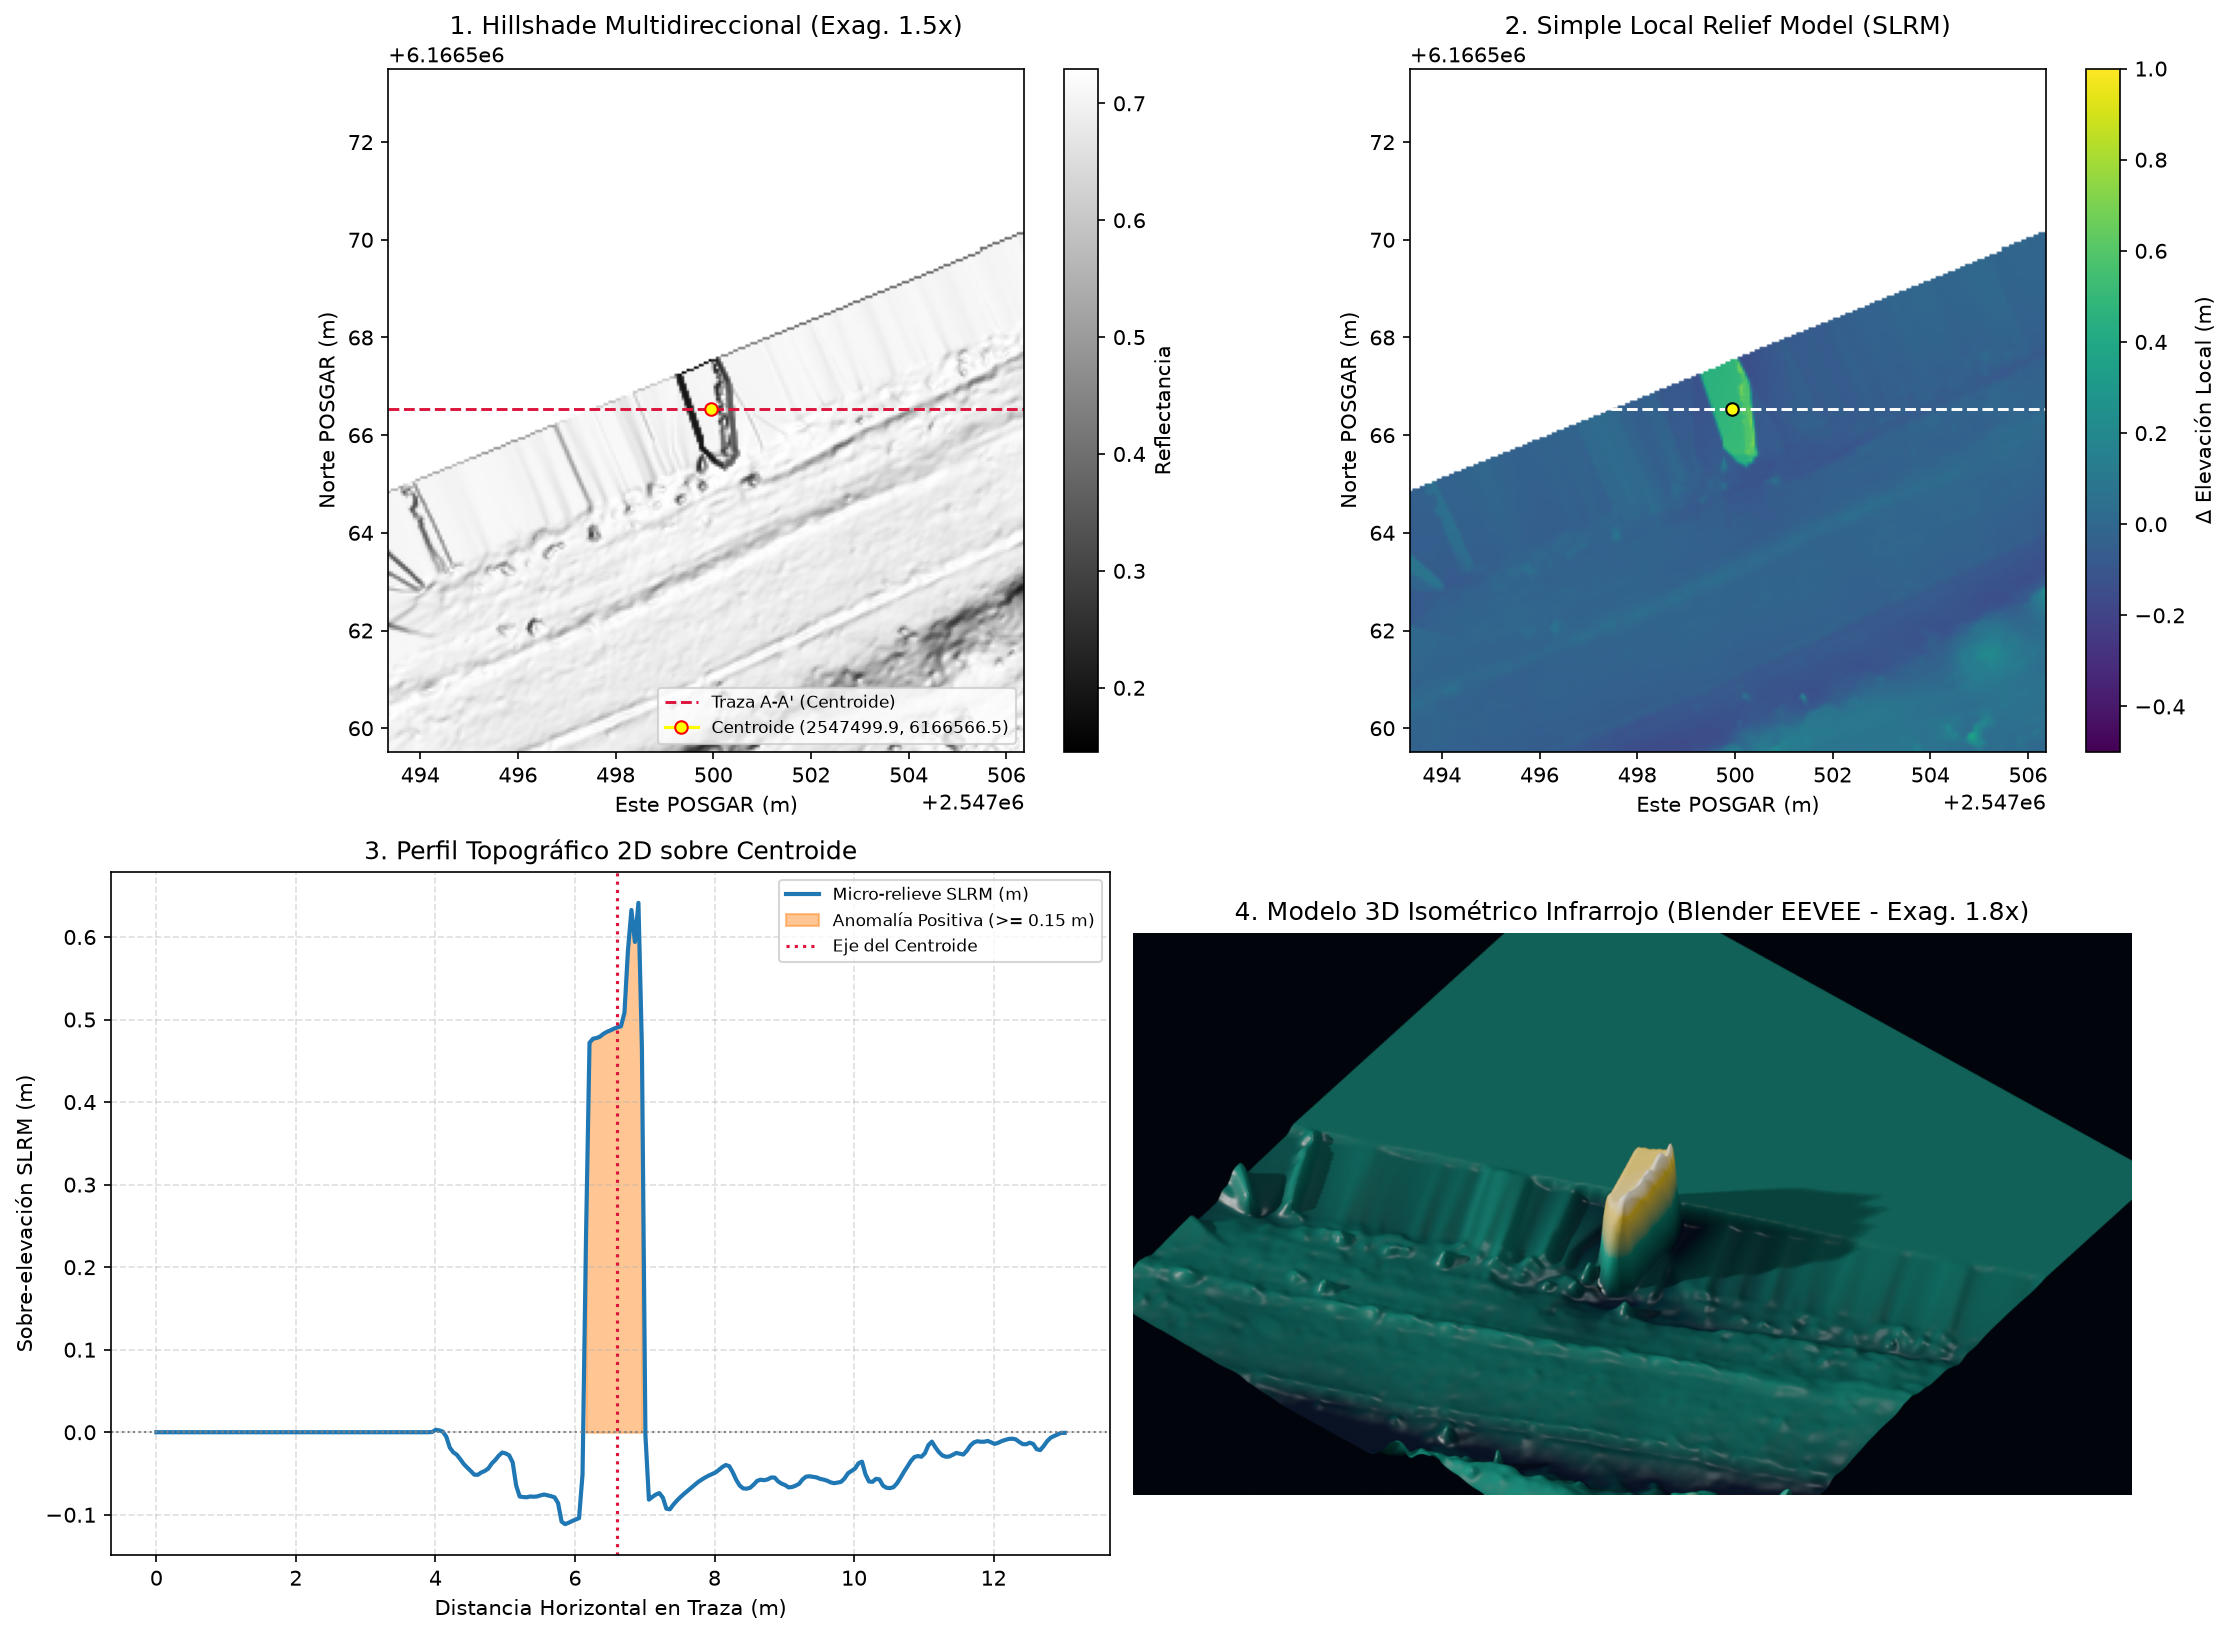
\includegraphics[width=\textwidth]{figures/fig6b_san_rafael_uav_5cm.png}
  \caption{Caso UAV sub-m\'etrico (\texttt{ARQ-HRM-0001}, San Rafael, \texttt{ZENODO:3383227}): prisma ortogonal de $1{,}24\,\mathrm{m}^2$ y huellas de rodado mec\'anico (\textbf{ARTEFACTO}, \emph{hail pad} HailPixel, certeza $98\%$).}
  \label{fig:hailpixel}
\end{subfigure}
\caption{Contraste multi-escala de l\'aminas periciales de 4 paneles con modelado 3D en Blender 4.2 EEVEE sobre ejemplos verificados y descartados.}
\label{fig:cases4panel}
\end{figure}

\subsection{F\'isica de Detectabilidad, Benchmark Nacional V1 y Calibrador ML}

La Figura~\ref{fig:physics}A demuestra la relaci\'on cuadr\'atica $A_{\min,\mathrm{eff}} = 2\cdot\mathrm{GSD}_{\mathrm{nativo}}^2$ que gobierna la detectabilidad f\'isica a lo largo de cuatro \'ordenes de magnitud espacial. Mientras un vuelo UAV de $0{,}05\,\mathrm{m/px}$ resuelve rasgos desde $0{,}005\,\mathrm{m}^2$ y un producto aerofotogram\'etrico IGN de $5\,\mathrm{m/px}$ alcanza estructuras desde $50\,\mathrm{m}^2$ (cubriendo gran parte de recintos andinos y casas-pozo grandes), un DEM satelital de $30\,\mathrm{m/px}$ impone un piso f\'isico de $1800\,\mathrm{m}^2$, dejando en la zona f\'isicamente irrecuperable a los parapetos patag\'onicos ($6$--$50\,\mathrm{m}^2$) y casas-pozo serranas ($12$--$80\,\mathrm{m}^2$). La proyecci\'on de los $121$ descartes emp\'iricos sobre este plano evidencia por qu\'e $98$ de los $133$ registros curados en \texttt{BENCHMARK\_V1\_DATASET.json} poseen \texttt{sensor\_detectable = False} al evaluarse sobre grilla satelital supermuestreada de $30\,\mathrm{m}$ (frente a $35$ con \texttt{sensor\_detectable = True}), validando la exclusi\'on del denominador computable y la activaci\'on de \texttt{INCONCLUSIVE} cuando se interrogan micro-estructuras por debajo del l\'imite de Nyquist geomorfol\'ogico.

\begin{figure}[htbp]
\centering
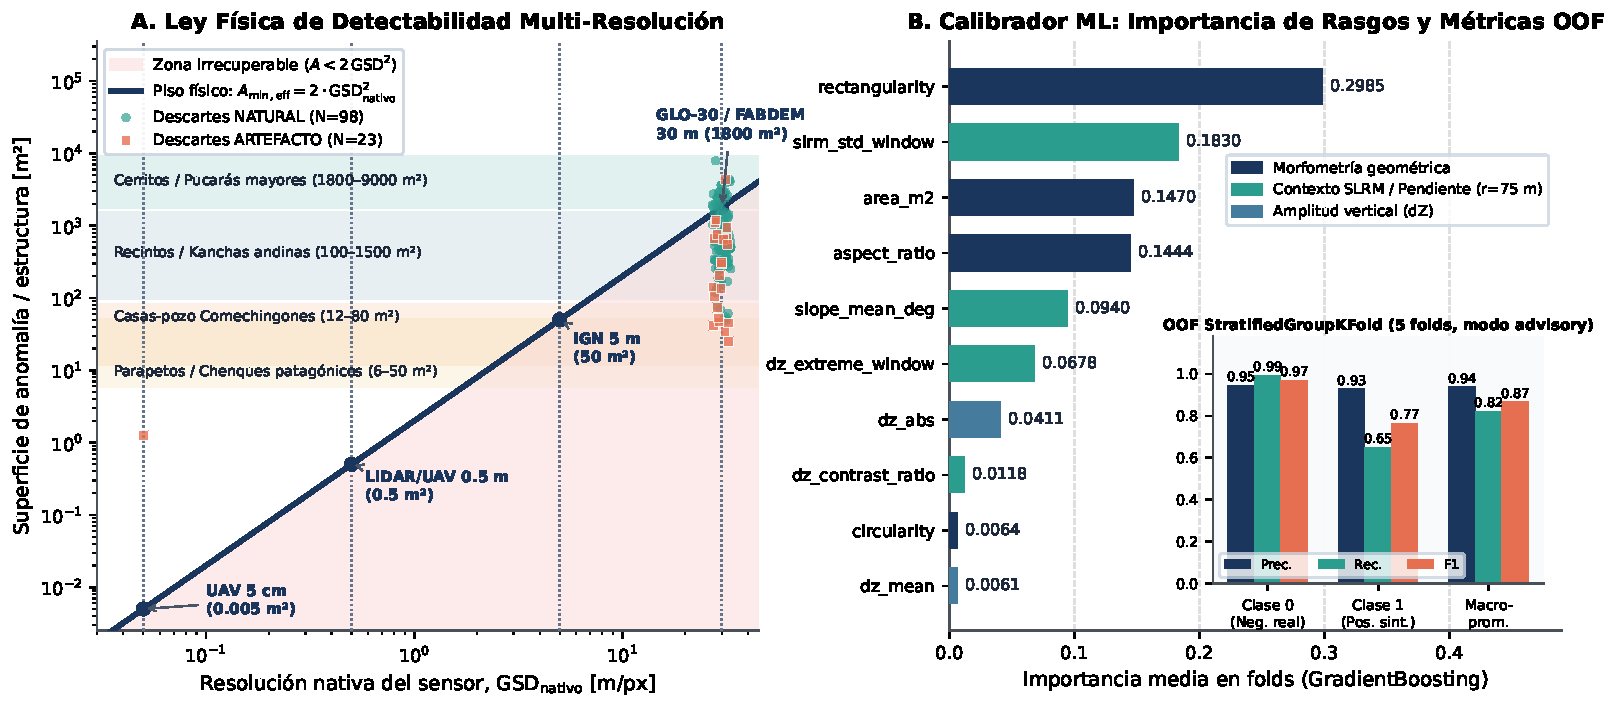
\includegraphics[width=\textwidth]{figures/fig3_scale_detectability_physics.pdf}
\caption{\textbf{A.} Ley f\'isica de detectabilidad $A_{\min,\mathrm{eff}} = 2\cdot\mathrm{GSD}_{\mathrm{nativo}}^2$ frente a los rangos caracter\'isticos de estructuras arqueol\'ogicas argentinas y la distribuci\'on emp\'irica de los $121$ descartes auditados. \textbf{B.} Importancia relativa de variables del calibrador \texttt{GradientBoostingClassifier} isot\'onico y m\'etricas \emph{out-of-fold} bajo \texttt{StratifiedGroupKFold} ($5$ particiones, $N=146$, modo \emph{advisory}).}
\label{fig:physics}
\end{figure}

Para el entrenamiento y diagn\'ostico del calibrador supervisado (\texttt{ML\_BENCHMARK\_METRICS.md}), se ensamblaron $N=146$ observaciones compuestas por $126$ \emph{hard negatives} reales de \texttt{DESCARTES\_VLM.json} (l\'inea base) y $20$ positivos sint\'eticos plantados sobre DTM de $0{,}5\,\mathrm{m/px}$ y $30\,\mathrm{m/px}$ con geometr\'ia conocida. En evaluaci\'on \emph{out-of-fold} con particionado espacialmente agrupado (\texttt{StratifiedGroupKFold}, $5$ folds), el modelo alcanz\'o los desempe\~nos resumidos en la Tabla~\ref{tab:ml_bench} y la Figura~\ref{fig:physics}B. La rectangularidad ($0{,}2985$), la desviaci\'on est\'andar SLRM de ventana ($0{,}1830$), el \'area ($0{,}1470$) y la raz\'on de aspecto ($0{,}1444$) explicaron el $77{,}3\%$ de la importancia agregada del modelo, mientras que \texttt{ndvi\_anomaly\_delta} present\'o importancia nula en esta versi\'on por ausencia de bandas \'opticas en corridas heredadas previas a la Fase 4.

\begin{table}[htbp]
\centering
\caption{M\'etricas \emph{out-of-fold} del calibrador ML (\texttt{StratifiedGroupKFold}, $5$ folds, $N=146$) y composici\'on auditada de \texttt{BENCHMARK\_V1\_DATASET.json}.}
\label{tab:ml_bench}
\footnotesize
\begin{tabularx}{\textwidth}{L{4.8cm} c c c Y}
\toprule
\multicolumn{5}{l}{\textbf{Panel A. Desempe\~no Out-of-Fold del Calibrador ML (Modo \emph{advisory} por sesgo de resoluci\'on sint\'etica)}} \\
\midrule
\textbf{Clase / Promedio} & \textbf{Precision} & \textbf{Recall} & \textbf{F1-Score} & \textbf{Observaci\'on Epist\'emica} \\
\midrule
Clase 0 --- \texttt{NATURAL / ARTEFACTO} ($n=126$) & $0{,}947$ & $0{,}992$ & $0{,}969$ & Controles negativos reales auditados por Juez VLM. \\
Clase 1 --- \texttt{ANTROPICA} sint\'etica ($n=20$) & $0{,}929$ & $0{,}650$ & $0{,}765$ & Estructuras plantadas ($0{,}5$ y $30\,\mathrm{m/px}$); mide separabilidad, no recall en campo. \\
\textbf{Macro-promedio} & \textbf{0,938} & \textbf{0,821} & \textbf{0,867} & Re-entrenable autom\'aticamente v\'ia \texttt{train\_calibrator()} al confirmar sitios reales. \\
\midrule
\multicolumn{5}{l}{\textbf{Panel B. Curadur\'ia Estructural de \texttt{BENCHMARK\_V1\_DATASET.json} ($133$ registros activos, $29$ bloques espaciales)}} \\
\midrule
\textbf{Nivel de Evidencia / Partici\'on} & \textbf{Cantidad} & \shortstack{\textbf{Confirm.}\\\textbf{arqueol.}} & \shortstack{\textbf{Elegible}\\\textbf{ciego}} & \textbf{Trazabilidad SHA-256 y Categor\'ias} \\
\midrule
\texttt{AI\_REJECTED\_CANDIDATE} & $124$ & \texttt{False} & \texttt{False} & Excluye $2$ sint\'eticos (\texttt{ARQ-0025}, \texttt{ARQ-0026}); fusiona $86$ atributos geomorfol\'ogicos sin duplicar. \\
\texttt{PUBLISHED\_SITE\_REFERENCE} & $9$ & \texttt{False} & \texttt{False} & Coordenadas p\'ublicas $\pm 100\,\mathrm{m}$ (\texttt{known\_sites\_published.csv}); excluidas de \texttt{blind\_test}. \\
\texttt{EXPERT\_REVIEWED} / \texttt{FIELD\_CONFIRMED} & $0$ & \texttt{True} & \texttt{True} & Reservadas para Etapas 5 y 6 bajo convenio institucional. \\
Bloques: \texttt{development} / \texttt{validation} / \texttt{blind\_test} & $99$ / $34$ / $0$ & --- & --- & Partici\'on por \texttt{region\_block\_id} \citep{Roberts2017}; \texttt{blind\_test} congelado en $0$. \\
\bottomrule
\end{tabularx}
\end{table}

Crucialmente, declaramos de forma expl\'icita un sesgo de resoluci\'on en el calibrador actual: los positivos sint\'eticos incluyen grillas de $0{,}5\,\mathrm{m/px}$, mientras que la mayor\'ia de los negativos provienen de GLO-30 ($30\,\mathrm{m/px}$). En pruebas internas, activar el calibrador en modo de bloqueo (\texttt{--ml-mode filter}) suprime candidatos v\'alidos en zonas satelitales nuevas; por ello, el sistema opera por defecto en modo consejero (\texttt{--ml-mode advisory}), aportando la probabilidad calibrada al contexto del Juez Pericial sin bloquear el an\'alisis morfom\'etrico. Asimismo, \texttt{BENCHMARK\_V1\_DATASET.json} consolida $133$ entradas verificadas por hashes SHA-256 de procedencia y mantiene \texttt{blind\_test = 0} hasta incorporar controles positivos reales bajo convenio institucional.

% ==================== SECTION 5 ====================
\FloatBarrier
\section{Protocolo Pre-registrado de Validaci\'on Externa (Etapas 4 y 5) y Marco \'Etico-Legal}

Para superar la circularidad de evaluar algoritmos \'unicamente con descartes de IA o coordenadas bibliogr\'aficas aproximadas ($\pm 100\,\mathrm{m}$), el proyecto pre-registr\'o un protocolo experimental cerrado previo al env\'io de material a especialistas externos (\texttt{docs/PROTOCOLO\_ETAPAS\_4\_Y\_5.md}) siguiendo las advertencias de \citet{Casana2021} y \citet{Vinci2024}.

\subsection{Etapa 4: Comparaci\'on Apareada Multi-Resoluci\'on por Bioma}

En la Etapa~4 se comparar\'an ventanas geogr\'aficas id\'enticas proyectadas en POSGAR 2007 a trav\'es de tres escalas espaciales nativas ($30\,\mathrm{m/px}$ GLO-30/MDE-Ar v2.1, $5\,\mathrm{m/px}$ fotogram\'etrico IGN y $0{,}05$--$1{,}0\,\mathrm{m/px}$ LiDAR/UAV) en al menos dos o tres biomas contrastantes (ej.\ NOA prepune\~no, piedemonte cuyano y Yungas o humedales litorales), prohibiendo promediar resultados entre biomas sin desglose (\texttt{by\_biome}). Se cuantificar\'an cuatro m\'etricas operativas: (1) tasa de persistencia inter-escala entre detecciones a $30\,\mathrm{m}$ y rasgos reales a $\le 5\,\mathrm{m}$, (2) sensibilidad estratificada en cuatro intervalos de superficie ($<50$, $50$--$500$, $500$--$1800$ y $\ge 1800\,\mathrm{m}^2$) con intervalos de confianza del $95\%$ de \citet{Wilson1927}, (3) desplazamiento medio de centroides $\Delta c$ e \'indice $\mathrm{IoU}$ espacial, y (4) densidad de falsas alarmas ($\mathrm{FP/km}^2$) antes y despu\'es de aplicar \texttt{should\_abstain\_prediction()}.

\subsection{Etapa 5: Evaluaci\'on Ciega Multi-Especialista y Reglas Estad\'isticas de Validez}

El m\'odulo \texttt{src/core/blind\_review.py} implementa un generador criptogr\'afico de paquetes de evaluaci\'on ciega (\texttt{export\_blind\_review\_pack}) que distingue estrictamente entre el \textbf{lote piloto exploratorio de calibraci\'on de instrumento} (actualmente generado con $12$ l\'aminas \texttt{BLIND-0001}..\texttt{BLIND-0012}, \texttt{seed=42}, \texttt{blind\_test=0}, destinado \'unicamente a verificar legibilidad y cegamiento) y el \textbf{lote confirmatorio independiente} futuro ($N \ge 60$ l\'aminas o m\'inimo piloto de $30$, estratificado $25\%$ controles positivos con precisi\'on $<15\,\mathrm{m}$ y $A \ge 2\cdot\mathrm{GSD}^2$, $25\%$ geoformas naturales dif\'iciles en $5$ subcategor\'ias, $25\%$ estructuras modernas/artefactos en $5$ subcategor\'ias, y $25\%$ detecciones algor\'itmicas in\'editas en bloques \texttt{blind\_test}).

\begin{figure}[htbp]
\centering
\begin{subfigure}[t]{0.94\textwidth}
  \centering
  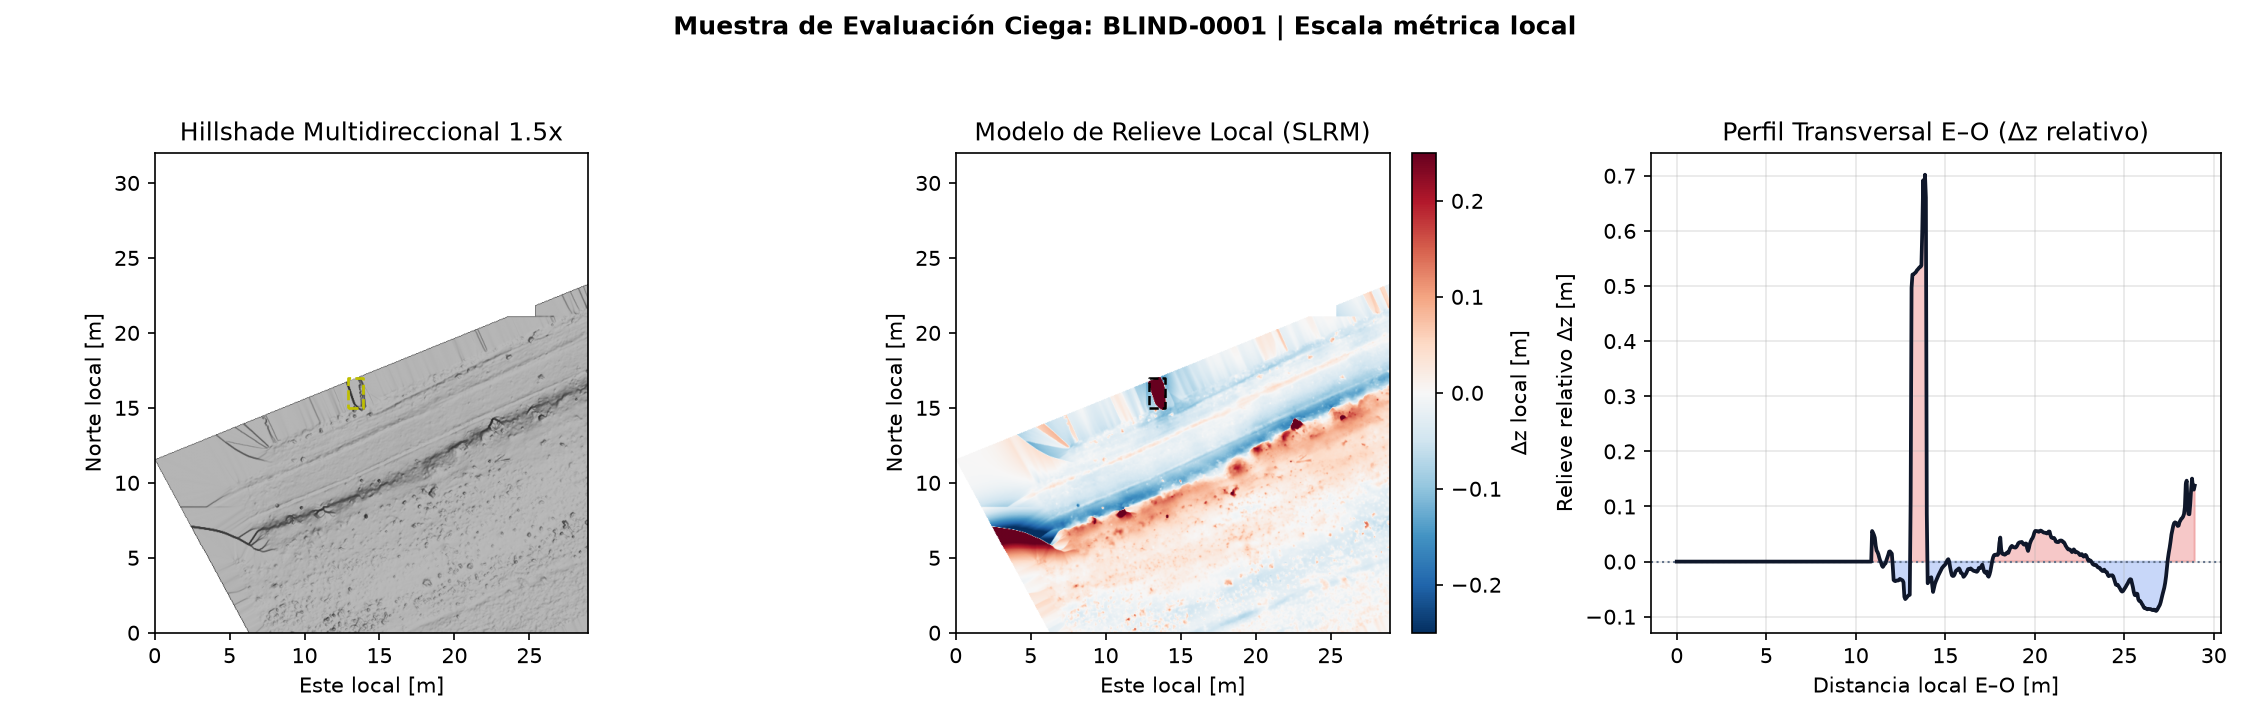
\includegraphics[width=\textwidth]{figures/fig7a_blind_0001.png}
  \caption{Muestra piloto \texttt{BLIND-0001} ($\mathrm{GSD}=0{,}05\,\mathrm{m/px}$, \texttt{cuyo\_monte}): ejes locales de $0$ a $30\,\mathrm{m}$ y relieve relativo $\Delta z$ centrado en la mediana.}
  \label{fig:blind1}
\end{subfigure}

\vspace{6pt}
\begin{subfigure}[t]{0.94\textwidth}
  \centering
  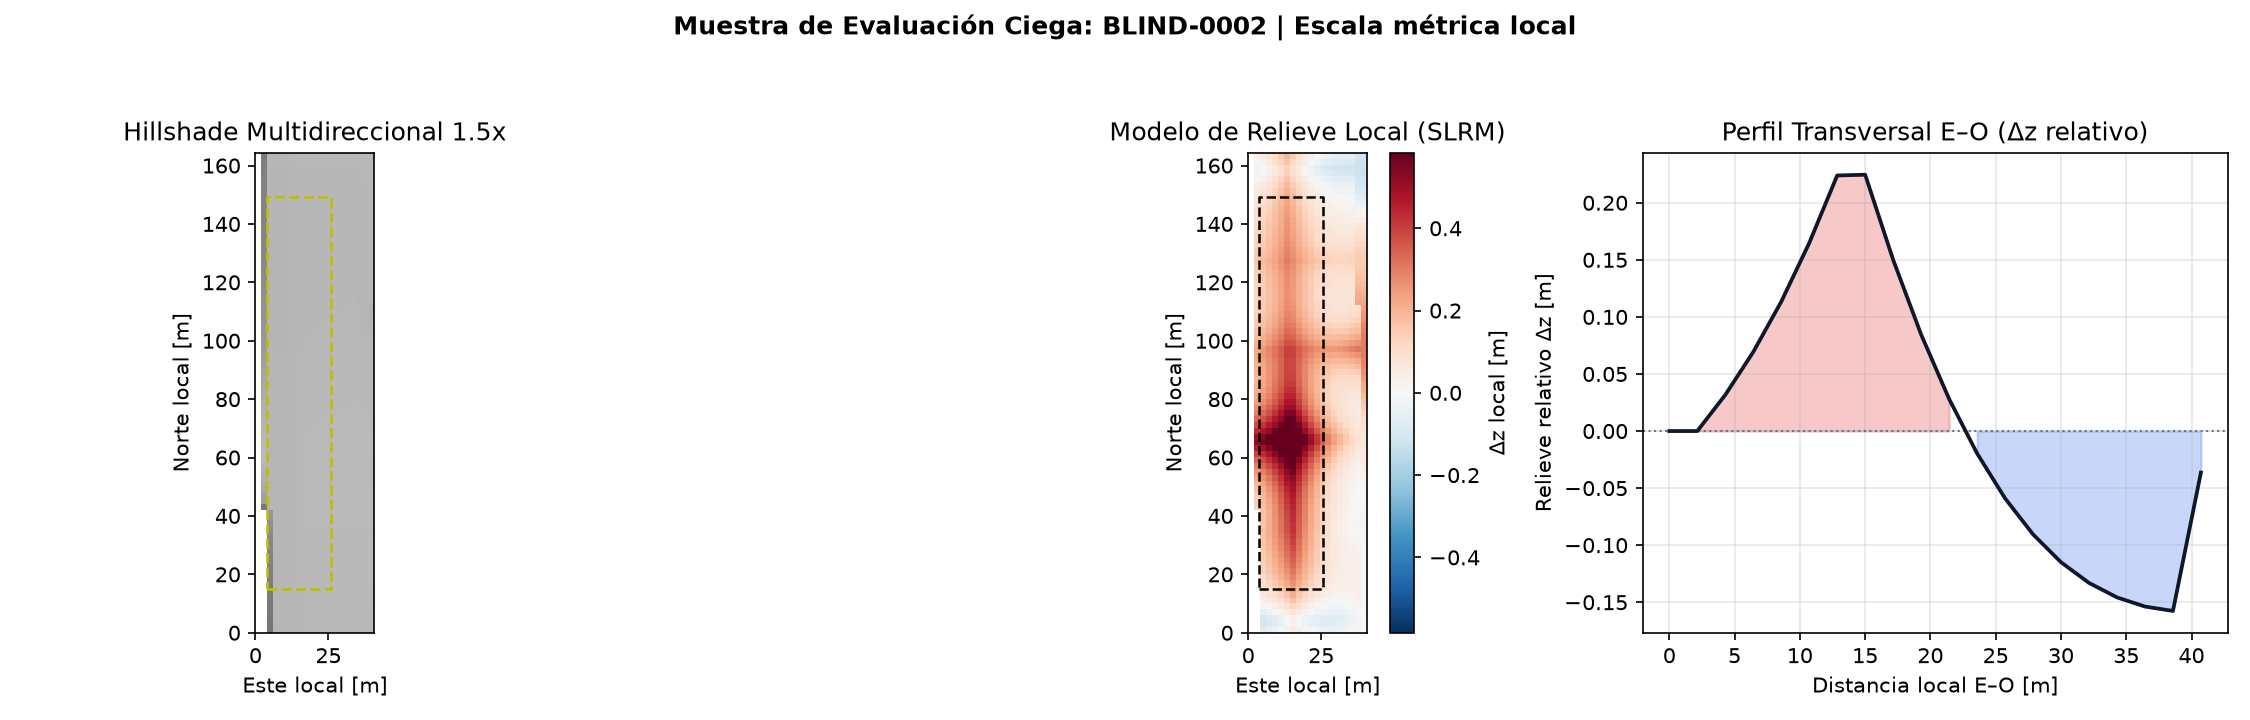
\includegraphics[width=\textwidth]{figures/fig7b_blind_0002.png}
  \caption{Muestra piloto \texttt{BLIND-0002} ($\mathrm{GSD}=2{,}0\,\mathrm{m/px}$, \texttt{meseta\_patagonica}): ventana local anonimizada sin coordenadas geod\'esicas ni scores IA.}
  \label{fig:blind2}
\end{subfigure}
\caption{Ejemplos reales del paquete piloto de evaluaci\'on ciega generados directamente desde GeoTIFF mediante \texttt{render\_blind\_candidate\_lamina()} y verificados con \texttt{strip\_png\_metadata\_and\_verify()} (cero etiquetas EXIF ni chunks PNG textuales).}
\label{fig:blind}
\end{figure}

Como ilustra la Figura~\ref{fig:blind}, cada l\'amina exhibe tres paneles sincr\'onicos (Hillshade $1{,}5\times$, SLRM y perfil E--O en relieve relativo $\Delta z$ centrado en la mediana para impedir inferir la cota absoluta sobre el nivel del mar) en ejes locales relativos $(0\ldots W\,\mathrm{m},\; 0\ldots H\,\mathrm{m})$. La funci\'on \texttt{strip\_png\_metadata\_and\_verify()} re-codifica cada imagen y audita la ausencia total de EXIF y de chunks PNG \texttt{tEXt}, \texttt{iTXt}, \texttt{zTXt}, \texttt{eXIf} y \texttt{tIME}, registrando sus hashes SHA-256 en \texttt{BLIND\_REVIEW\_PACK\_MANIFEST.json} y aislando la correspondencia en \texttt{CONFIDENTIAL\_BLIND\_KEY.json}.

Al menos $2$--$3$ especialistas acreditados independientes clasifican cada \'item en cuatro categor\'ias cerradas (\texttt{ARCHAEOLOGICAL\_PLAUSIBLE}, \texttt{NATURAL\_GEOFORM}, \texttt{MODERN\_INFRASTRUCTURE}, \texttt{INCONCLUSIVE}), escala ordinal de plausibilidad ($1$--$4$) y confianza Likert ($1$--$5$). El protocolo declara \textbf{v\'alido} el experimento \'unicamente si concurren: (i) $100\%$ de integridad SHA-256 y borrado de metadatos; (ii) tasa de respuesta $\ge 90\%$; (iii) concordancia nominal $\kappa_{\mathrm{Fleiss/Cohen}} \ge 0{,}40$ (moderada en \citealp{LandisKoch1977}; \citealp{Cohen1960,Fleiss1971}) y concordancia ordinal cuadr\'atica $\kappa_{\mathrm{cuad}} \ge 0{,}60$ (sustancial); y (iv) ausencia de degeneraci\'on marginal (prevalencia por clase $\le 85\%$). Si en una combinaci\'on sensor/bioma $\kappa < 0{,}20$ o los dict\'amenes humanos \texttt{INCONCLUSIVE} superan el $50\%$, el protocolo la declara morfol\'ogicamente no resoluble. Un candidato transita a \texttt{EXPERT\_REVIEWED} s\'olo con consenso $\ge 2/3$ en \texttt{ARCHAEOLOGICAL\_PLAUSIBLE}, severidad ordinal $\ge 3$ y ning\'un voto firme de infraestructura moderna ($\ge 4$).

\subsection{Hoja de Ruta Progresiva (Etapas 0--7) y Gobernanza Institucional}

La Tabla~\ref{tab:roadmap} resume el avance verificado en las Etapas~0 a 3 y el programa interinstitucional articulado con \textbf{INAPL}, \textbf{FFyL-UBA}, \textbf{IMHICIHU-CONICET}, \textbf{IGN} y \textbf{AAPRA} para ejecutar las Etapas~4 a 7 dentro de un horizonte de seis meses bajo plena observancia de la Ley N\textsuperscript{o}~25.743.

\begin{table}[htbp]
\centering
\caption{Plan maestro de validaci\'on progresiva en 8 etapas (24 semanas) y compuertas de verificaci\'on.}
\label{tab:roadmap}
\footnotesize
\begin{tabularx}{\textwidth}{c L{4.2cm} L{2.4cm} Y}
\toprule
\textbf{Etapa} & \textbf{Foco Cient\'ifico-T\'ecnico} & \textbf{Estado Actual} & \textbf{Puerta de Aprobaci\'on / Evidencia Verificada} \\
\midrule
\textbf{0} & L\'inea base, fuente \'unica de verdad y estados & \textbf{Implementada} & \texttt{CAMPAIGN\_MANIFEST.json}, \texttt{BASELINE\_REPORT\_V1.md}, 7 estados y \texttt{CLAIMS\_REGISTRY}. \\
\textbf{1} & Auditor\'ia del motor (\texttt{DEMQualityProfile}, SVF/Openness) & \textbf{Implementada} & $8/8$ pruebas deterministas aprobadas (\texttt{test\_engine\_scientific\_audit.py}). \\
\textbf{2} & Benchmark V1 por bloques espaciales & \textbf{Implementada} & $133$ registros curados en $29$ bloques, $10$ clases de negativos dif\'iciles, \texttt{blind\_test = 0}. \\
\textbf{3} & Calibraci\'on ML, abstenci\'on y paquete ciego & \textbf{Implementada} & Abstenci\'on integrada en pipeline/MCP; \texttt{blind\_review.py} y piloto $12$ l\'aminas operativos. \\
\textbf{4} & Contraste apareado $30\,\mathrm{m}$ vs.\ $5\,\mathrm{m}$ vs.\ $<1\,\mathrm{m}$ & Protocolo cerrado & Convenio IGN/CONICET/UBA: persistencia, recall estratificado e IoU en $2$--$3$ biomas. \\
\textbf{5} & Evaluaci\'on ciega multi-especialista & Protocolo cerrado & $\kappa_{\mathrm{Fleiss/Cohen}} \ge 0{,}40$, $\kappa_{\mathrm{cuad}} \ge 0{,}60$, IC Wilson $95\%$ y auditor\'ia de desacuerdos. \\
\textbf{6} & Contraste autorizado en terreno (arts.\ 23--24) & Planificada & Inspecci\'on de campo bajo permisos vigentes hacia estado \texttt{FIELD\_CONFIRMED}. \\
\textbf{7} & Cierre reproducible V2.0 y publicaci\'on conjunta & Planificada & Liberaci\'on de m\'etricas agregadas y pesos calibrados con resguardo estricto de coordenadas. \\
\bottomrule
\end{tabularx}
\end{table}

% ==================== SECTION 6 ====================
\FloatBarrier
\section{Discusi\'on: Alcance Cient\'ifico, Limitaciones y Ciencia Secundaria}

\subsection{Frontera de Afirmaciones Permitidas (\texttt{CLAIMS\_REGISTRY})}

El aporte distintivo de \textbf{ArchaeoLiDAR-AR} no reside en prometer descubrimientos autom\'aticos milagrosos desde im\'agenes orbitales de $30\,\mathrm{m}$, sino en formalizar en c\'odigo una frontera epist\'emica auditable. El proyecto sostiene emp\'iricamente cinco capacidades: (1) ingesta geod\'esica reproducible por \emph{Range Requests} en POSGAR 2007; (2) detecci\'on de anomal\'ias de doble signo con piso f\'isico de 2 p\'ixeles nativos; (3) cribado catastral frente a IGN, OSM y sitios publicados; (4) generaci\'on de l\'aminas multimodales $4/6$ paneles con Blender 3D y trazabilidad forense; y (5) aislamiento confidencial de localizaciones sensibles. Rec\'iprocamente, el propio sistema proh\'ibe afirmar sin validaci\'on externa de las Etapas~4--6: (a) descubrimiento aut\'onomo de sitios arqueol\'ogicos confirmados; (b) detectabilidad de muros finos o casas-pozo $<1800\,\mathrm{m}^2$ sobre DEM de $30\,\mathrm{m/px}$; (c) interpretaci\'on de scores morfol\'ogicos o ML como probabilidad arqueol\'ogica calibrada en terreno; y (d) emisi\'on de acusaciones legales autom\'aticas de huaqueo sin peritaje institucional competente.

\subsection{Implicaciones del Piso de Escala y Reutilizaci\'on Geomorfol\'ogica}

Los resultados de la campa\~na nacional ($98$ geoformas naturales y $23$ artefactos descartados sobre $121$ anomal\'ias, con $0$ derivaciones a campo) confirman en territorio sudamericano las advertencias formuladas por \citet{Casana2014} y \citet{Vinci2024}: a resoluci\'on satelital global de $30\,\mathrm{m/px}$, las geoformas coluviales, domos volc\'anicos y albardones fluviales producen firmas topogr\'aficas equivalentes en escala a macro-recintos y cerritos cuando se inspeccionan sin perfil 2D, contexto espectral ni control de piso f\'isico. La integraci\'on de cortes transversales, Blender 3D y bandas Sentinel-2 L2A redujo la carga de falsas alarmas derivadas a cero antes de incurrir en costos de campa\~na. Adicionalmente, la conservaci\'on estructurada de los descartes en \texttt{INVENTARIO\_GEOMORFOLOGICO.geojson} ($n=81$ geoformas tipificadas en $11$ categor\'ias) transforma un residuo tradicionalmente desechado de la prospecci\'on arqueol\'ogica en un activo abierto para estudios de hidrogeolog\'ia, remoci\'on en masa, geomorfolog\'ia glaciar y din\'amica fluvial.

\subsection{Limitaciones Actuales y Trabajo Futuro}

Se identifican tres limitaciones concretas que orientan la transici\'on hacia la versi\'on 2.0: (1) ausencia de positivos arqueol\'ogicos reales confirmados en terreno dentro de \texttt{BENCHMARK\_V1\_DATASET.json} (\texttt{FIELD\_CONFIRMED = 0}), lo que obliga a mantener el calibrador ML en modo \texttt{advisory}; (2) desajuste de resoluci\'on entre positivos sint\'eticos ($0{,}5\,\mathrm{m/px}$) y negativos GLO-30 en el entrenamiento ML, que se resolver\'a incorporando las coberturas de $5\,\mathrm{m/px}$ del IGN y vuelos LiDAR/UAV argentinos en Etapa~4; y (3) necesidad de integrar cobertura de radar de apertura sint\'etica (SAR / Sentinel-1) para penetrar nubosidad persistente en las Yungas y Selva Paranaense cuando el canal \'optico de Fase 4 presente cobertura nubosa elevada.

% ==================== SECTION 7 ====================
\section{Conclusiones}

\textbf{ArchaeoLiDAR-AR} demuestra que es factible construir una plataforma nacional reproducible de teledetecci\'on arqueol\'ogica que integre eficiencia computacional (lectura parcial \texttt{/vsicurl/} en POSGAR 2007), rigor f\'isico multi-escala ($A_{\min,\mathrm{eff}} = 2\cdot\mathrm{GSD}_{\mathrm{nativo}}^2$), modelado morfol\'ogico \emph{NaN-safe} en doble polaridad, juicio pericial multimodal, aprendizaje supervisado con negativos dif\'iciles, protocolo ciego libre de sesgos y resguardo geod\'esico alineado con la Ley Nacional N\textsuperscript{o}~25.743. Verificado por $64/64$ pruebas autom\'aticas (incluyendo $8/8$ auditor\'ias f\'isico-geoespaciales deterministas) y respaldado por una campa\~na depurada de $121$ anomal\'ias con $0$ falsas alarmas derivadas a campo y $81$ geoformas inventariadas, el sistema y su protocolo pre-registrado de Etapas~4 y 5 quedan disponibles para iniciar colaboraci\'on interinstitucional con arque\'ologos y organismos de patrimonio en Argentina.

% ==================== BACK MATTER ====================
\FloatBarrier
\section*{Disponibilidad de C\'odigo, Datos y Reproducibilidad}

El c\'odigo fuente del servidor FastMCP, la suite de pruebas (\texttt{64} tests), el esquema \texttt{benchmark\_v1\_schema.json}, las m\'etricas agregadas (\texttt{CAMPAIGN\_MANIFEST.json}, \texttt{ML\_BENCHMARK\_METRICS.md}), los protocolos pre-registrados y el script generador de figuras (\texttt{docs/paper/generate\_figures.py}) est\'an disponibles bajo licencia MIT en \url{https://github.com/pmtempone/argentina_history_arq}. La verificaci\'on local y la ejecuci\'on de campa\~na se reproducen mediante:

\begin{tcolorbox}[colback=codebg,colframe=slateborder,boxrule=0.5pt,arc=2pt,left=6pt,right=6pt,top=4pt,bottom=4pt]
\raggedright\ttfamily\footnotesize
cd archaeo-lidar-mcp \&\& python3 -m venv venv\\
source venv/bin/activate \&\& pip install -e \textquotedbl{}.[dev]\textquotedbl{}\\
./venv/bin/pytest -v \hfill \# 64/64 pruebas autom\'aticas\\
./venv/bin/python -m src.autonomous\_prospector {-}{-}target ZONA\_23\_DELTA\_PARANA {-}{-}max-candidates 4\\
./venv/bin/python scripts/build\_campaign\_manifest.py \hfill \# Consolida BASELINE\_REPORT\_V1.md\\
./venv/bin/python ../docs/paper/generate\_figures.py \hfill \# Regenera Figuras 2, 3 y 4
\end{tcolorbox}

Los archivos \texttt{*ANEXO\_CONFIDENCIAL\_COORDENADAS.json}, \texttt{*CONFIDENTIAL\_BLIND\_KEY.json} y \texttt{*MAPA\_PROSPECCION\_*.geojson} se encuentran excluidos del repositorio p\'ublico mediante \texttt{.gitignore} y disponibles \'unicamente bajo convenio institucional conforme a la Ley N\textsuperscript{o}~25.743.

\section*{Consideraciones \'Eticas y Cumplimiento Legal}

Este estudio no realiz\'o intervenciones invasivas ni excavaciones en terreno. Todo procesamiento se ejecut\'o sobre teledetecci\'on satelital abierta y el conjunto UAV meteorol\'ogico p\'ublico \texttt{ZENODO:3383227} \citep{Soderholm2019}. Los nueve sitios de referencia incluidos en \texttt{known\_sites\_published.csv} corresponden exclusivamente a monumentos hist\'oricos o sitios tur\'isticos de acceso p\'ublico con coordenadas aproximadas ($\pm 100\,\mathrm{m}$). Cualquier prospecci\'on de campo futura derivada de la Etapa~6 requerir\'a autorizaci\'on previa de la autoridad competente (INAPL / direcciones provinciales de patrimonio, arts.\ 23--24 de la Ley N\textsuperscript{o}~25.743).

\section*{Transparencia en el Uso de Inteligencia Artificial y Conflictos de Inter\'es}

Los modelos de aprendizaje autom\'atico (\texttt{GradientBoostingClassifier}) y de lenguaje/visi\'on multimodal (\texttt{vlm\_judge.py}) fueron utilizados exclusivamente como herramientas auxiliares de clasificaci\'on y cribado preliminar sobre l\'aminas topogr\'aficas, documentando sus dict\'amenes en \texttt{DESCARTES\_VLM.json} con abstenci\'on formal de cualquier afirmaci\'on arqueol\'ogica aut\'onoma sin revisi\'on ciega humana. El autor declara no tener conflictos de inter\'es financieros ni institucionales y se\~nala que el proyecto ha sido desarrollado de manera abierta e independiente sin financiamiento comercial espec\'ifico.

\bibliographystyle{apalike}
\bibliography{references}

\end{document}
